\chapter{Mes réalisations}
\label{Réalisations}

    Nous allons maintenant explorer mes contributions concrètes au projet MoCapIA.
    Même si le projet est assez performant, simple d'utilisation et rapide, les erreurs totales observées à la fin du processus restent trop importantes pour une analyse biomécanique sérieuse et une utilisation dans le domaine sportif. En traçant la distance entre deux points (ex : hanche droite et genou droit) au cours d'un mouvement, la valeur fluctue énormément et des valeurs aberrantes sont observées. Voici un graphe représentant la distance entre les deux points cités précédemment au cours d'un mouvement de squat : on observe une variation de $\pm 40mm$ pour une distance qui devrait théoriquement rester constante. 
    \begin{figure}[h]
        \centering
        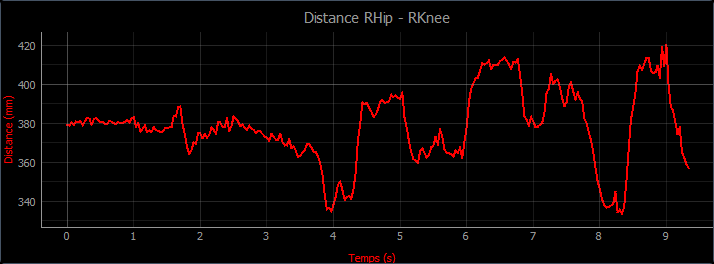
\includegraphics[width=0.8\textwidth]{assets/Capture d'écran process/resultFinDeStage/DEBUTSTAGEDistance_RHip_-_RKnee_.png}
        \caption{Distance entre hanche droite et genou droit – début de stage}
        \label{fig:distance_hip_knee_debut_stage} 
    \end{figure}
    Ce sont des erreurs trop importantes et la suite du chapitre va se focaliser sur les mesures prises pour améliorer la précision et la stabilité du système.

    Mais avant tout, il est d'abord nécessaire de comprendre d'où viennent les erreurs. Comme expliqué préalablement, MoCapIA se décompose en 3 étapes principales : la calibration, l'estimation 2D et la triangulation. Chacune de ces étapes peut engendrer des erreurs. Il est donc primordial d'analyser chacune de ces étapes pour comprendre où se situent les principales sources d'erreurs. Voici le plan que nous allons suivre dans ce chapitre :
    \begin{itemize}
        \item \textbf{TEST 0 - Analyse de l'effet du damier sur la calibration :} dans ce test, l'objectif est d'analyser l'impact du damier en utilisant différentes configurations (taille des carreaux, nombre de carreaux).
        \item \textbf{TEST 1 - Analyse de l'homogénéisation de la calibration :} on cherche cette fois à mesurer la précision de la calibration à différents endroits de la zone de capture en isolant les erreurs liées à l'estimation 2D (IA).
        \item \textbf{TEST 2 - Analyse de l'estimation 2D par l'IA :} ici, l'objectif est de mesurer les erreurs liées à l'estimation 2D en utilisant le système Vicon comme référence.
    \end{itemize}   
    Enfin, nous essayerons d'apporter différentes solutions pour améliorer la précision globale du système.
    
    \begin{figure}[H]
        \centering
        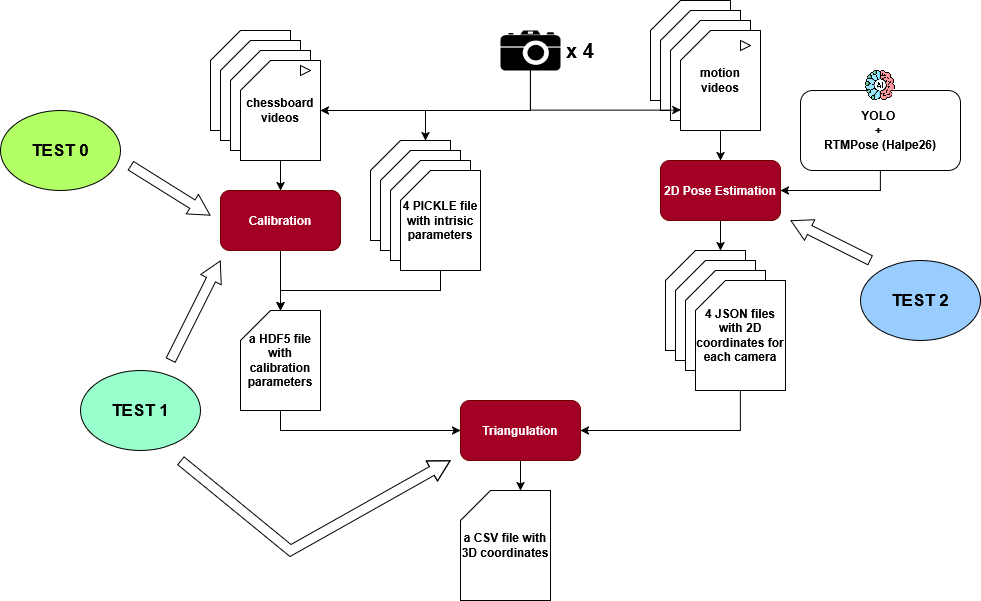
\includegraphics[width=\textwidth]{assets/Capture d'écran process/general/synthèseMOCAPIA_tests.drawio.png}
        \caption{Schéma récapitulatif des tests effectués}
        \label{fig:synthese_tests_mocapia}
    \end{figure}

\section{Analyse des erreurs liées à la calibration}

    La calibration et la triangulation sont les étapes mathématiques de base, mais essentielles pour notre logiciel ; il était important d'en connaître la précision et donc mesurer les erreurs qui sont liées à ces étapes. Pour ça il a fallu les isoler des erreurs liées à l'estimation 2D (traitées juste après).
    Pour l'étude suivante, on part de l'hypothèse suivante : dans un scénario théorique idéal (calibration et détection sans erreurs), la méthode DLT est exacte. Elle ne génère aucun biais ni erreur résiduelle intrinsèque (0 mm). L'erreur de reconstruction observée en pratique provient exclusivement de la propagation des incertitudes d'entrée (bruit de détection 2D et imprécisions de calibration) et non de la formulation mathématique de la DLT elle-même \cite{Triangulation}. Il est donc possible d'isoler les erreurs liées à la calibration même si on est capable d'observer les erreurs seulement après la triangulation.

    \subsection{TEST 0 - Analyse de l'effet du damier sur la calibration}

        Cette première analyse vise à mesurer l'impact du damier utilisé pour la calibration. Deux paramètres sont à étudier : la taille des carreaux qui composent le damier ainsi que leur nombre. Pour ça, 4 damiers de tailles différentes ont été fabriqués avec l'aide du FabLab (voir figure \ref{fig:damiers_fablab}) :
        \begin{itemize}
            \item Damier A : 7x6 carreaux de 120 mm
            \item Damier B : 7x6 carreaux de 100 mm
            \item Damier C : 10x9 carreaux de 85 mm
            \item Damier D : 10x9 carreaux de 60 mm.
        \end{itemize}

        Mais pour pouvoir comparer la calibration, il faut pouvoir exécuter le même mouvement à chaque fois. Pour ça, un bras articulé UR3 (\ref{fig:robot_articulé}) capable de reproduire exactement le même mouvement à chaque itération a été utilisé. En fixant les différents damiers sur le robot, il est maintenant possible de comparer la calibration obtenue avec chaque damier. 
        \begin{figure}[h]
            \centering % Pour centrer l'image
            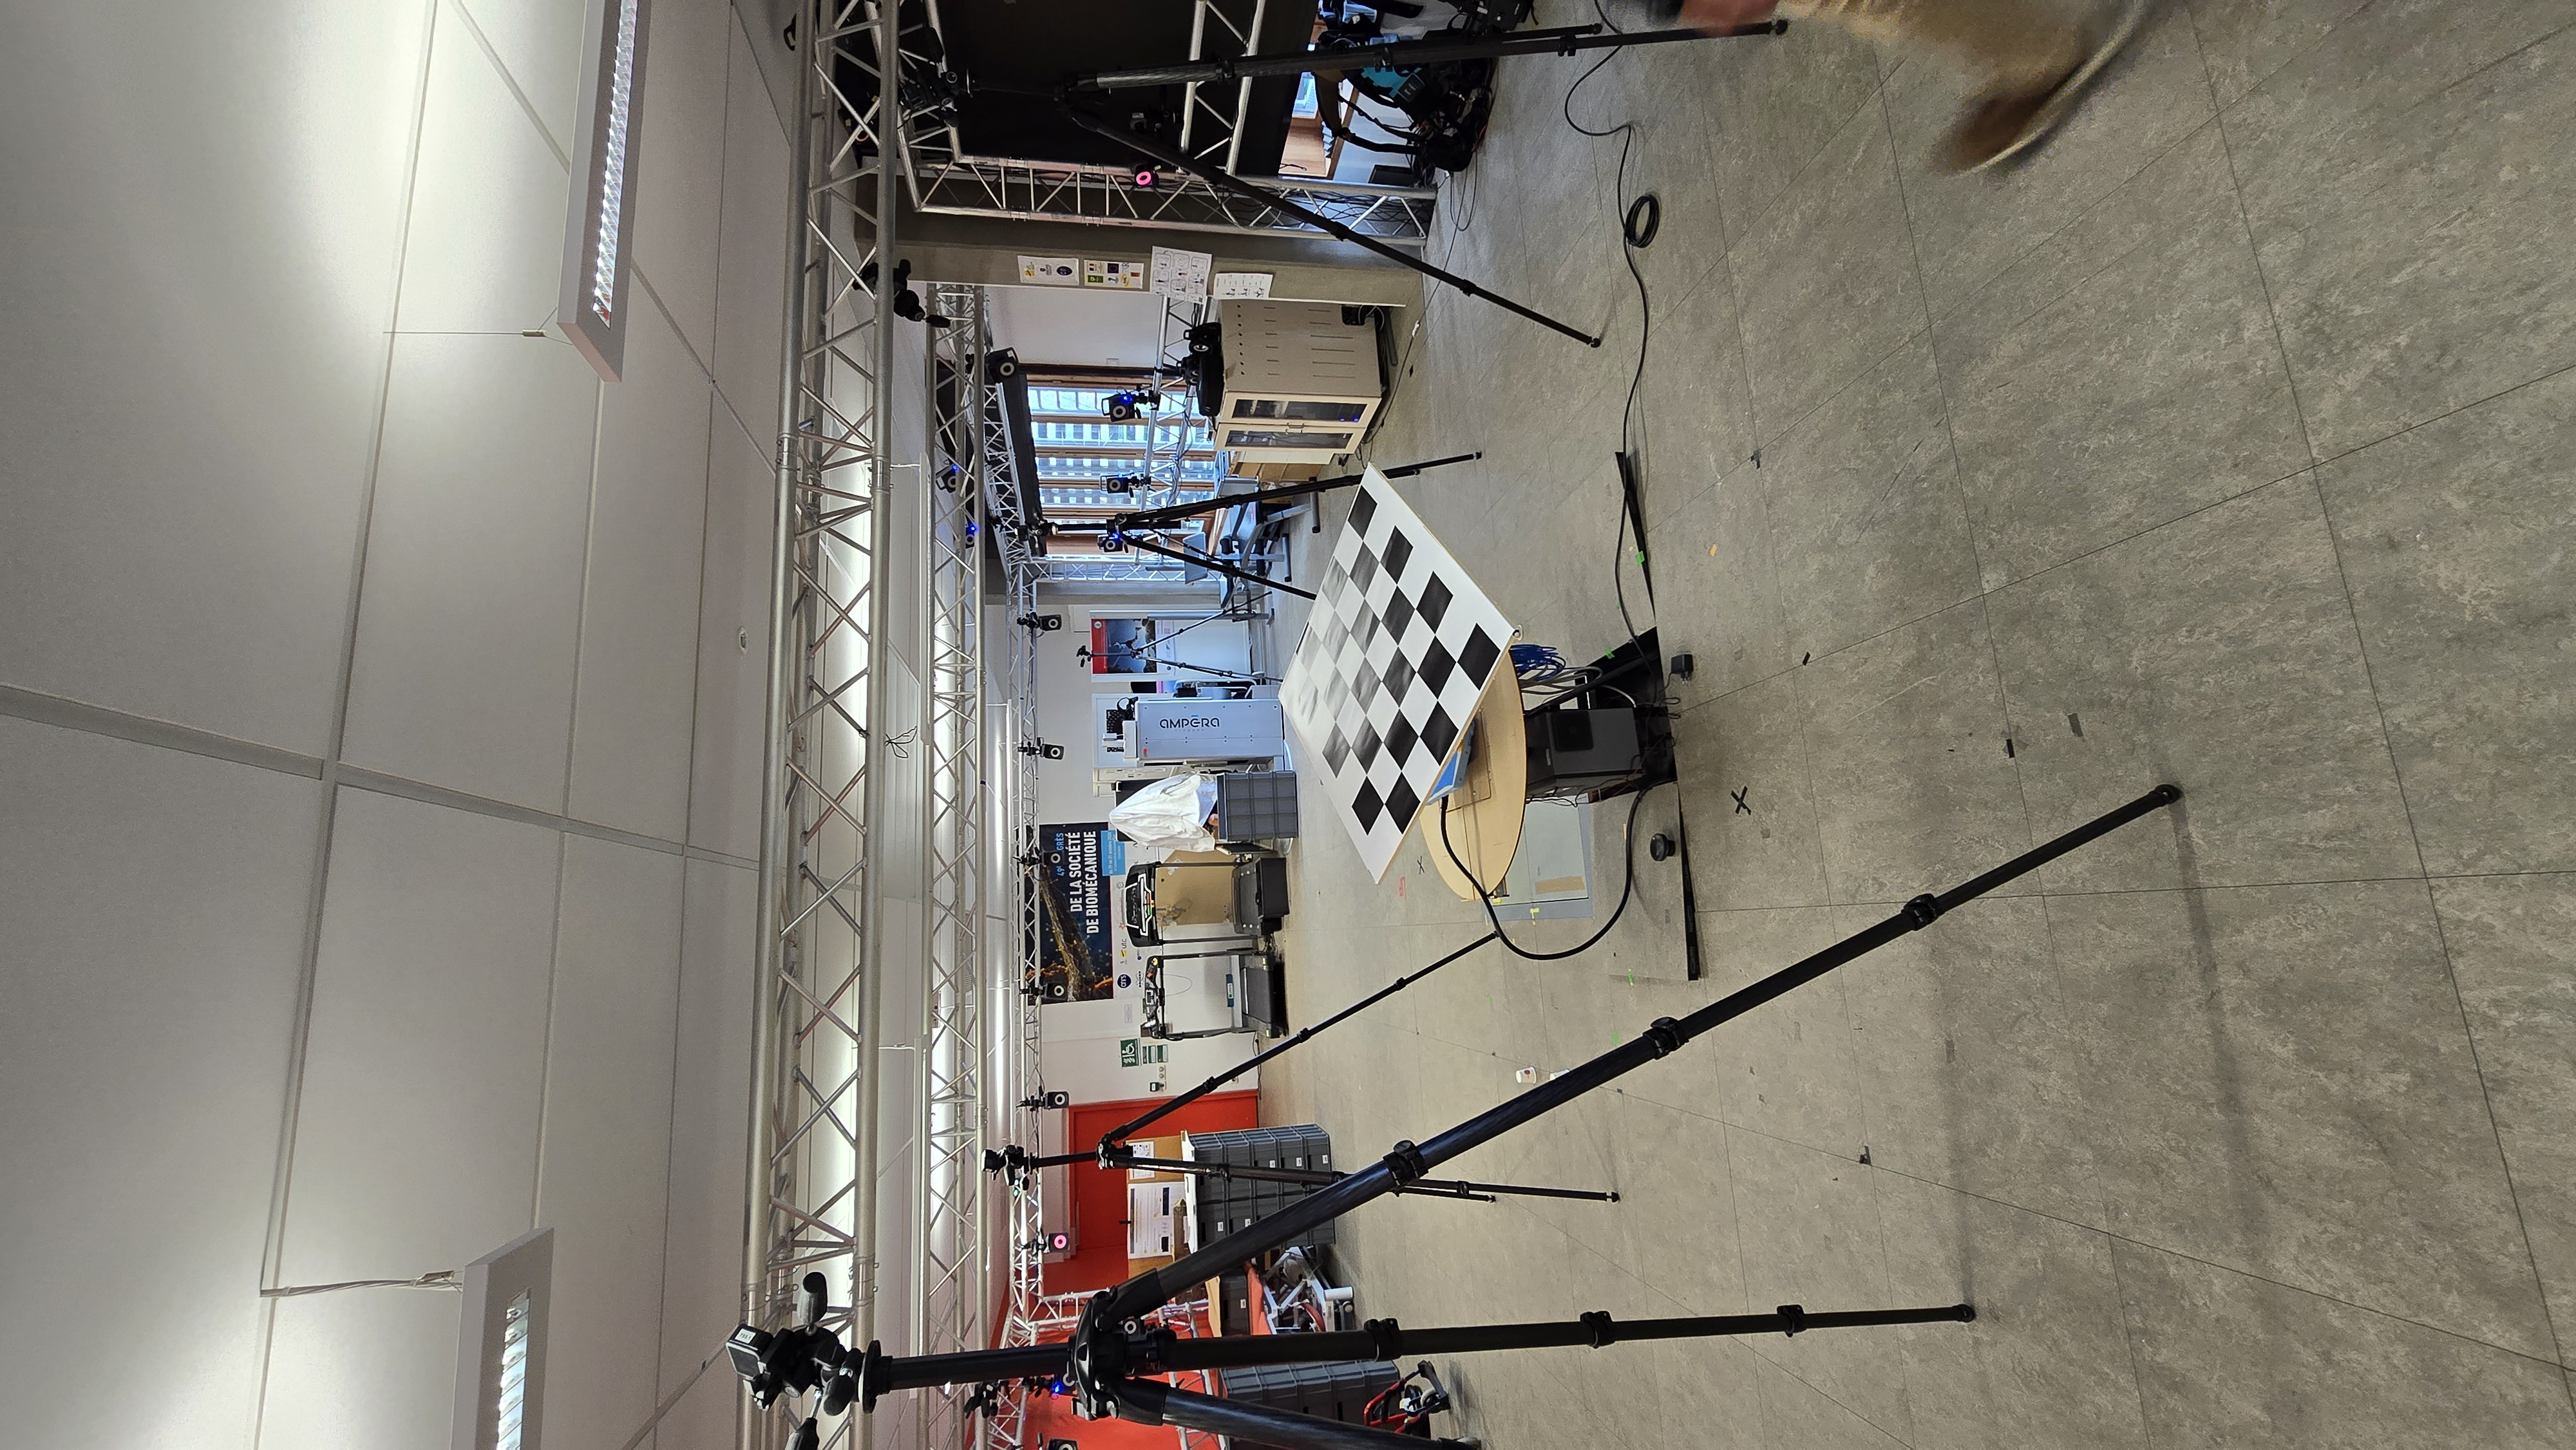
\includegraphics[width=0.8\textwidth, angle=-90]{assets/Capture d'écran process/Test_Damiers/scene_robot.jpg}
            \caption{Scène de calibration avec le bras articulé}
            \label{fig:scène_robot}
        \end{figure}

        Les résultats ci-dessous ont été obtenus pour un mouvement de rotation du bras de 360 degrés. En utilisant la table ANOVA (Analyse de la Variance), on est capable de répondre à la question : \textit{"Est-ce que le fait de changer de damier change réellement la mesure, ou est-ce juste du hasard ?"}. Sur la table ANOVA, on observe que la valeur \textit{p value} est proche de zéro ($7.25671e^{-286}$) sur un jeu de donnée de $1389$ points par damier. Cette valeur signifie que le choix du damier à un impact significatif sur la précision et la qualité de la calibration. À l'aide de la fonction MATLAB \texttt{multcompare()} appliqué à la mesure du Bras gauche (segment ElbowL - ShoudlerL), on est capable de savoir quels damiers sont statistiquement différents les uns des autres en les séparant en différents groupes. Un groupe s'impose comme étant statistiquement proche, celui du damier 7x6 100 mm et 10x9 60 mm. La moyenne de ce groupe $\mu \approx 266 mm$ est validé par le fait qu'avec deux damiers de géométrie différente, les résultats sont proches. Les damiers 7x6 120 mm et 10x9 85 mm semblent sur-estimé la longueur du membre. En effet, la distance du bras du sujet étant de $d_bras = 270 mm$, les résultats de ces deux damiers sont considérés par le calcul ANOVA comme trop éloigné statistiquement pour que cet écart soit uniquement dû au bruit.
        \begin{figure}[H]
            \centering
            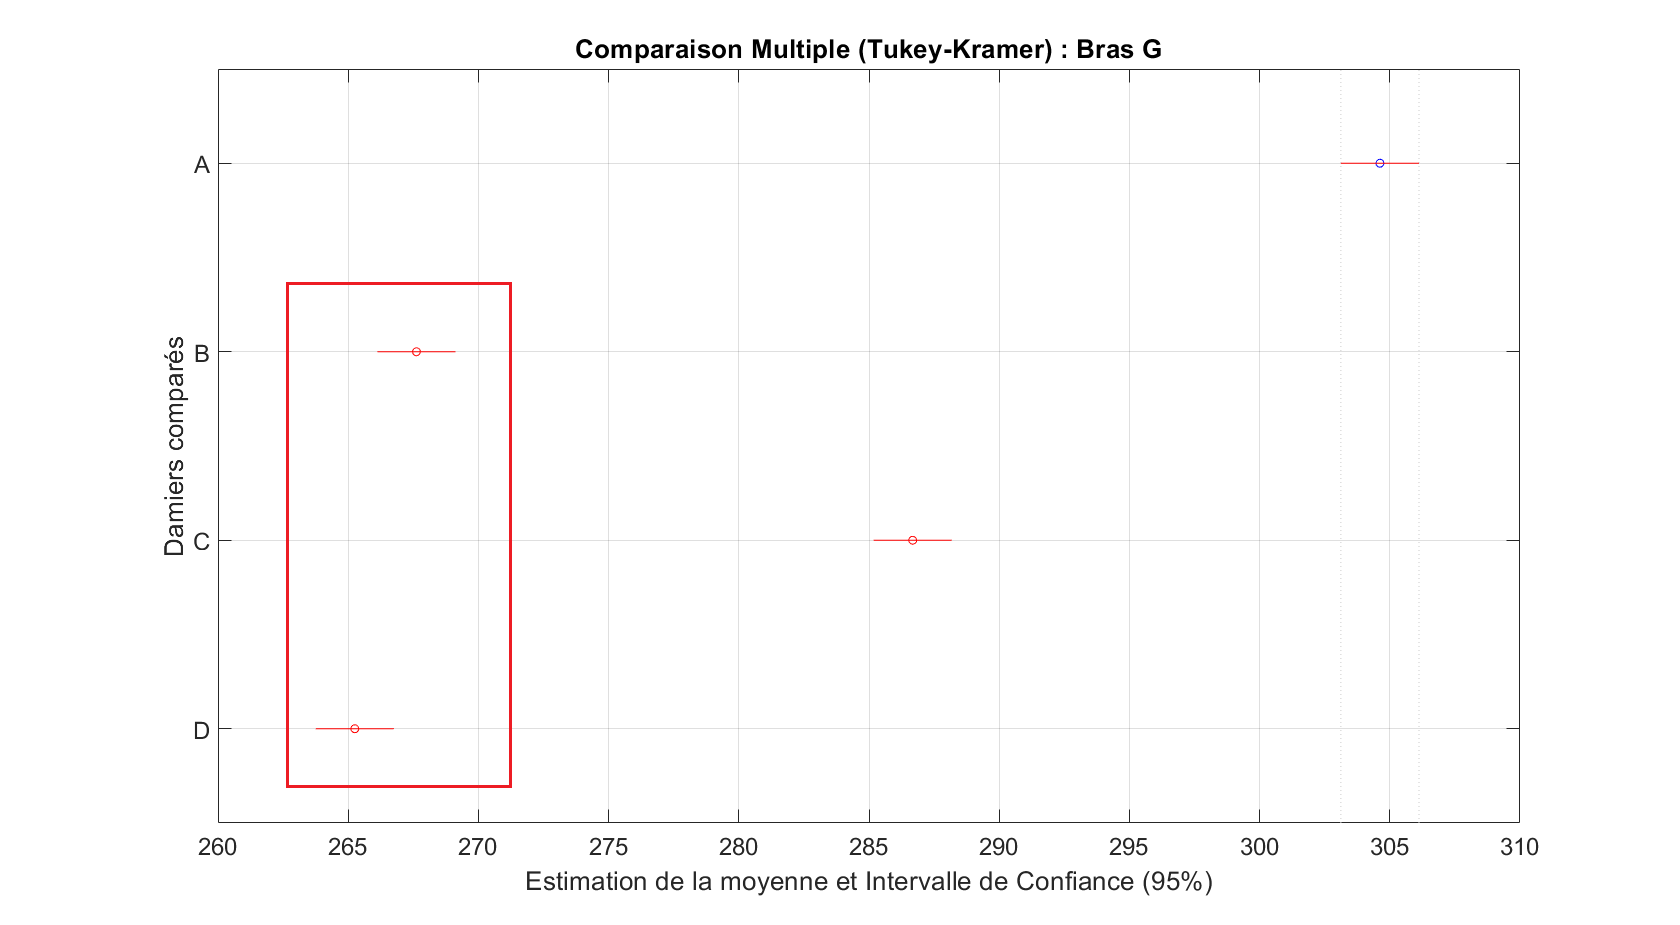
\includegraphics[width=\textwidth]{assets/Capture d'écran process/Test_Damiers/result_brasG.png}
            \caption{Graphique multcompare MATLAB des damiers}
            \label{fig:multcompare_damiers}
        \end{figure}

        Il a été décidé de compléter cette étude en observant la stabilité des résultats. Pour ça, une analyse \textit{boxplots} permet de conclure que la stabilité est bien plus forte avec le damier 10x9 60 mm et le damier 7x6 100 mm en plus d'être proche statistiquement parlant (\ref{boxplot_damiers}). Au contraire les damiers 7x6 120 mm et 10x9 85 mm présentent des quartiles plus écartés.
        \begin{figure}[H]
            \centering
            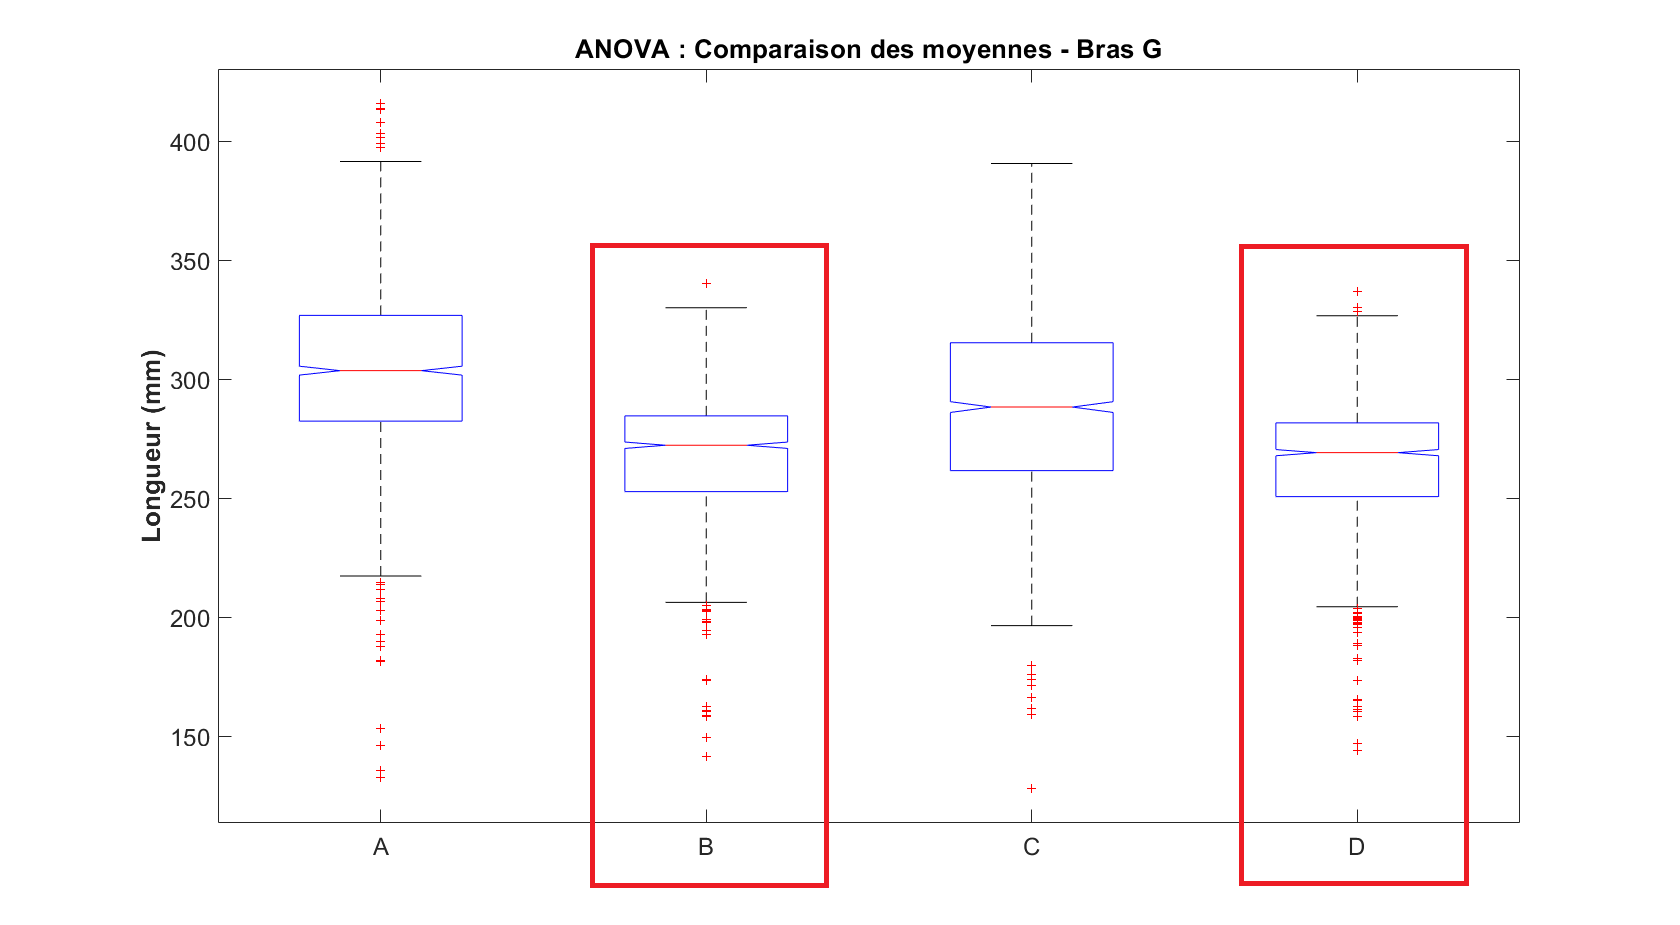
\includegraphics[width=\textwidth]{assets/Capture d'écran process/Test_Damiers/anova_boxplots_brasG.png}
            \caption{Boxplots sur la distance ElbowL - ShoulderL pour chaque damier}
            \label{boxplot_damiers}
        \end{figure}
        
        En conclusion, on remarque deux choses :
        \begin{itemize}
            \item Le nombre de carreaux n'a pas directement d'impact sur la précision de la calibration. En exemple, le damier 10x9 85 mm n'obtient pas de meilleurs résultats que le damier 7x6 100 mm ou 120 mm.
            \item La taille des carreaux n'a pas non plus un impact sur la calibration, car le damier 7x6 120 mm ne fait pas mieux que le damier 7x6 100 mm et le damier 10x9 85 mm ne fait pas mieux que le damier 10x9 60 mm.
            \item C'est plutôt la taille globale du damier qui a un impact sur la calibration. En effet, le damier 7x6 100 mm a une aire $A_1 \approx 0.42 m^2$ et le damier 10x9 60 mm a une aire $A_2 \approx 0.32 m^2$. Ces deux damiers sont ceux qui offrent les meilleurs résultats. À l'inverse, le damier 7x6 120 mm ($A_3 \approx 0.60 m^2$) et le damier 10x9 85 mm ($A_4 \approx 0.65 m^2$) sont ceux qui offrent les moins bons résultats. Ces résultats permettent d'émettre l'hypothèse que la \textbf{distorsion}, qui est plus importante sur les bords de l'image (appelé \textit{fisheye}), impacte fortement les résultats de la calibration \cite{CalibrationWeng}. En effet, en ayant un damier trop grand, les points caractéristiques situés sur les bords de l'image sont plus affectés par la distorsion, ce qui dégrade la calibration. Même si la distorsion est corrigée lors de la triangulation, elle ne l'est pas lors de la calibration. Pour utiliser un damier plus grand, il faudrait appliquer une correction de la distorsion lors de la calibration.
        \end{itemize}
        Pour la suite du projet, l'équipe a donc décidé d'utiliser le damier 7x6 100 mm qui offre un bon compromis entre précision et stabilité.

    \subsection{TEST 1 - Analyse de l'homogénéisation de la calibration}

        Maintenant que le damier est choisi, il est important de connaître la précision de la calibration. L'objectif ici est de mettre de côté les erreurs liées à l'estimation 2D pour se concentrer uniquement sur les erreurs liées à la calibration (nous avons vu dans l'introduction que la triangulation n'engendrait pas d'erreurs). Les coordonnées 2D utilisées seront obtenues à l'aide d'un clic-souris, précis au pixel (soit une précision) près grâce au zoom. Pour ça, une baguette de calibration a été utilisée contenant 3 points caractéristiques espacés de distances connues :
        \begin{itemize}
            \item Point 1 - Point 2 : 250 mm
            \item Point 2 - Point 3 : 243 mm
            \item Point 3 - Point 1 : 290 mm
        \end{itemize}
        La scène de test est représentée sur la figure \ref{fig:scène_verif_calib} ci-dessous. 
        \begin{figure}[H]
            \centering
            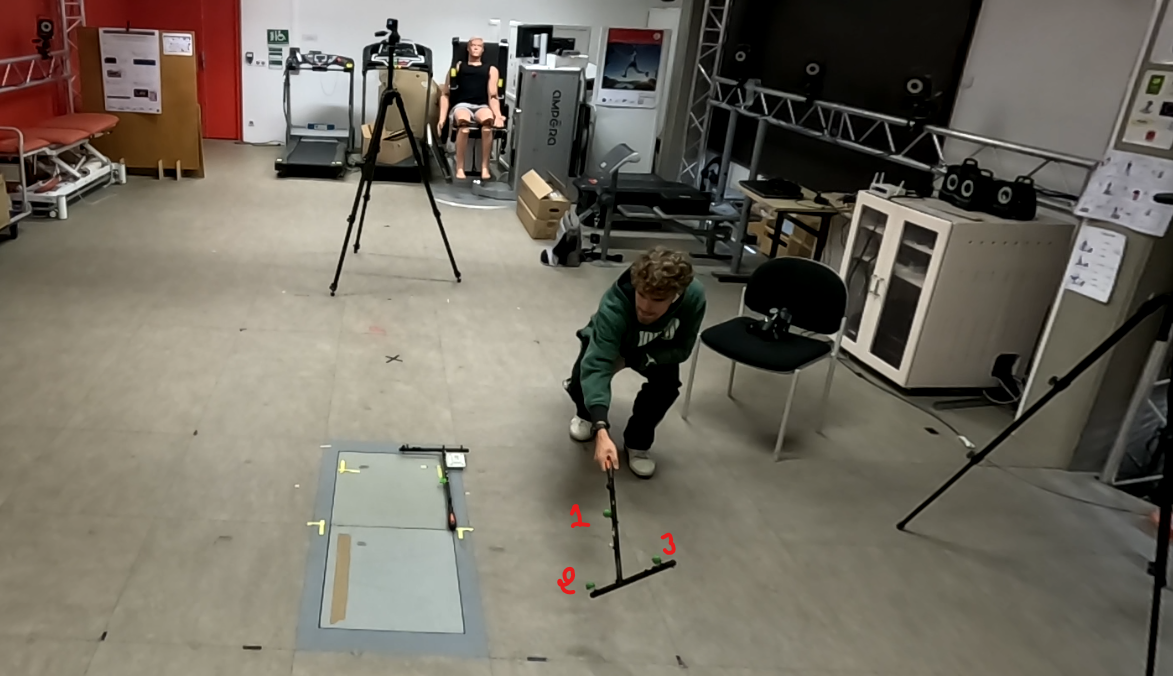
\includegraphics[width=0.8\textwidth]{assets/Capture d'écran process/Précision_CalibTriangulation/image.png}
            \caption{scène de vérification de points 3D}
            \label{fig:scène_verif_calib} % Une étiquette pour y faire référence
        \end{figure}
        \FloatBarrier
        Après avoir cliqué sur les 3 points caractéristiques à travers les 4 points de vue, les points triangulés (3D) sont comparés aux distances théoriques.
        Les erreurs sont représentées sur la figure \ref{fig:plot_calib_triang} qui représente la scène dans l'espace avec les caméras ainsi que les points caractéristiques de la baguette à plusieurs endroits dans la scène.
        \begin{figure}[H]
            \centering
            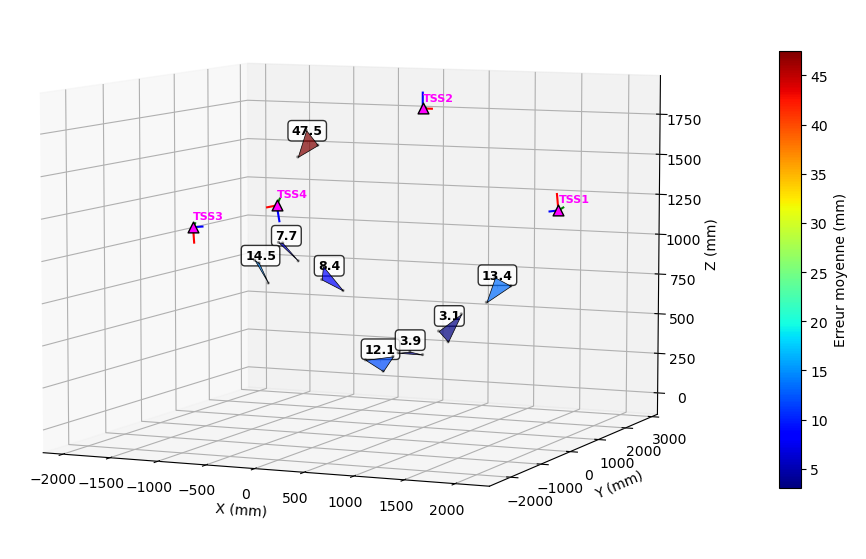
\includegraphics[width=0.8\textwidth]{assets/Capture d'écran process/Précision_CalibTriangulation/Figure_Calib.png}
            \caption{Résultat des erreurs de calibration après triangulation des 3 points caractéristiques}
            \label{fig:plot_calib_triang} % Une étiquette pour y faire référence
        \end{figure}
        
        La médiane des valeurs est de $8.4mm$. Cela représente une erreur relative de seulement $3.36\%$ pour une distance théorique de $250mm$. Étant donné que les erreurs totales observées précédemment étaient de l'ordre de la dizaine de centimètres, les résultats sont satisfaisants. 
        Cependant, certaines valeurs aberrantes ont été observées ($\approx 47.5mm$). Elles se situent proche des bords de la zone de capture. Cela indique donc que la précision de la calibration n'est pas totalement \textbf{homogène} sur l'ensemble de la zone commune (zone de capture). C'est donc un détail à prendre en compte lors du positionnement des caméras, mais aussi lors du mouvement du sujet.
        
        Finalement, pour un mouvement situé au centre de la zone de capture, \textbf{la calibration et la triangulation n'engendrent que très peu d'erreurs} sur le processus global. Une étude sur une autre méthode de triangulation (globale au lieu de locale) a été réalisée, mais n'a pas été concluante. Les résultats obtenus sont présentés en Annexe \ref{AnnexTriangu}.


\section{TEST 2 - Analyse de l'estimation 2D par l'IA}
\label{estimation2D}
    Pour rappel, nous utilisons deux modèles d'intelligence artificielle pour l'estimation 2D des points caractéristiques du corps humain : \textbf{YOLO} et \textbf{RTMPose}.
    En introduction, il avait été observé que des erreurs d'une dizaine de centimètres sur les longueurs des membres. De plus, la conclusion précédente permet d'affirmer que la majorité des erreurs proviennent de l'estimation 2D. Pour confirmer cette analyse, il faut calculer la précision et les erreurs liées à cette partie du processus. Pour ça on dispose d'un des systèmes les plus performants et précis qui existe : le Vicon. Précis à quelques millimètres près, il sera utilisé comme référence. Pour valider le résultat, il faut donc capturer les points caractéristiques du corps humain à la fois avec le Vicon, à la fois avec le MoCapIA et il va falloir comparer la distance entre chaque point 3D.
    Ce test a été réalisé en collaboration avec des étudiants en TX (Juliette Lafont et Dorian Biot). Sur la figure \ref{fig:yolo_rtmpose_vicon}, on peut voir la détection des points en 2D par YOLO (la boîte) et RTMPose (le squelette à 26 points) et éventuellement distinguer les marqueurs Vicon (les points lumineux blanc).

    \begin{figure}[H]
        \centering
        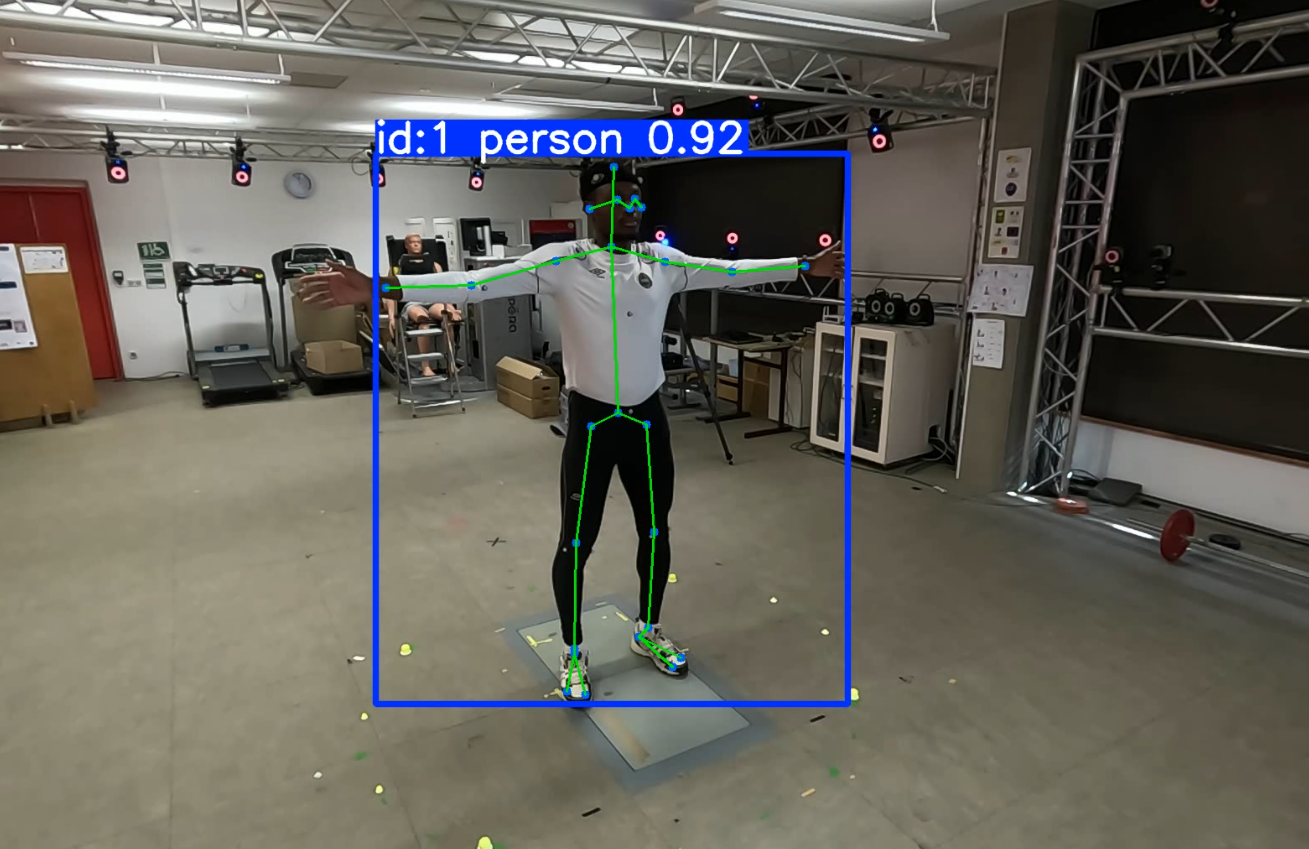
\includegraphics[width=\textwidth]{assets/Capture d'écran process/TX_ViconVSMocapIA/yolo_rtmpose.png}
        \caption{Marqueurs virtuels de MoCapIA et marqueurs physiques du Vicon}
        \label{fig:yolo_rtmpose_vicon}
    \end{figure}
    
    L'objectif de ce test est de comparer les deux systèmes de capture de mouvement (MoCapIA et Vicon) mais comme distinguer sur la figure \ref{fig:superposition_vicon_mocapia}, les marqueurs détectés par le Vicon ne correspondent pas tous aux points caractéristiques détectés par MoCapIA. Il est donc nécessaire de faire une correspondance entre les deux systèmes en calculant le milieu entre certains points Vicon. Un décalage constant est donc inévitable, mais il est quand même possible de comparer les deux systèmes en analysant la variation des mesures.

    \begin{figure}[H]
        \centering
        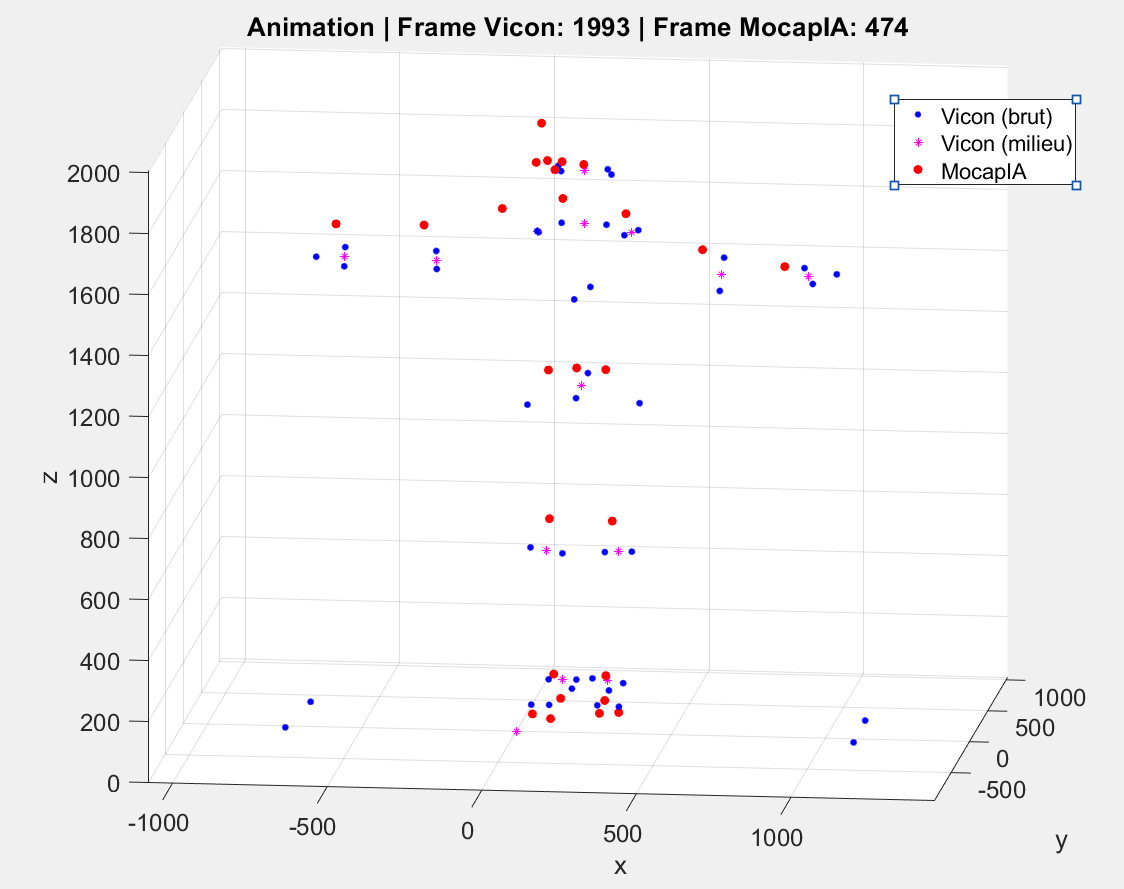
\includegraphics[width=\textwidth]{assets/Capture d'écran process/TX_ViconVSMocapIA/vicon_mocap_superpose.png}
        \caption{Superposition des points caractéristiques MoCapIA et Vicon pour l'étude qui va suivre}
        \label{fig:superposition_vicon_mocapia}
    \end{figure}

    Choisit par les TX comme un mouvement impliquant le haut du corps comme le bas, une séquence de quatre jumpings jacks à différentes vitesses a été enregistrée simultanément par le système Vicon et par le système MoCapIA.
    Venant de deux systèmes différents, les données doivent être synchronisées. Lors de chaque vidéo, le sujet part d'une \textit{T-pose} (position en T), effectue un "clap" avec les mains et en repérant la distance minimum entre les deux poignets, le système est capable d'initialiser un nouveau $t_{0}$ (voir figure \ref{fig:before_sync} et \ref{fig:sync}). 
    
    \begin{figure}[H]
    \centering
    % Première sous-figure
    \begin{subfigure}{\textwidth}
        \centering
        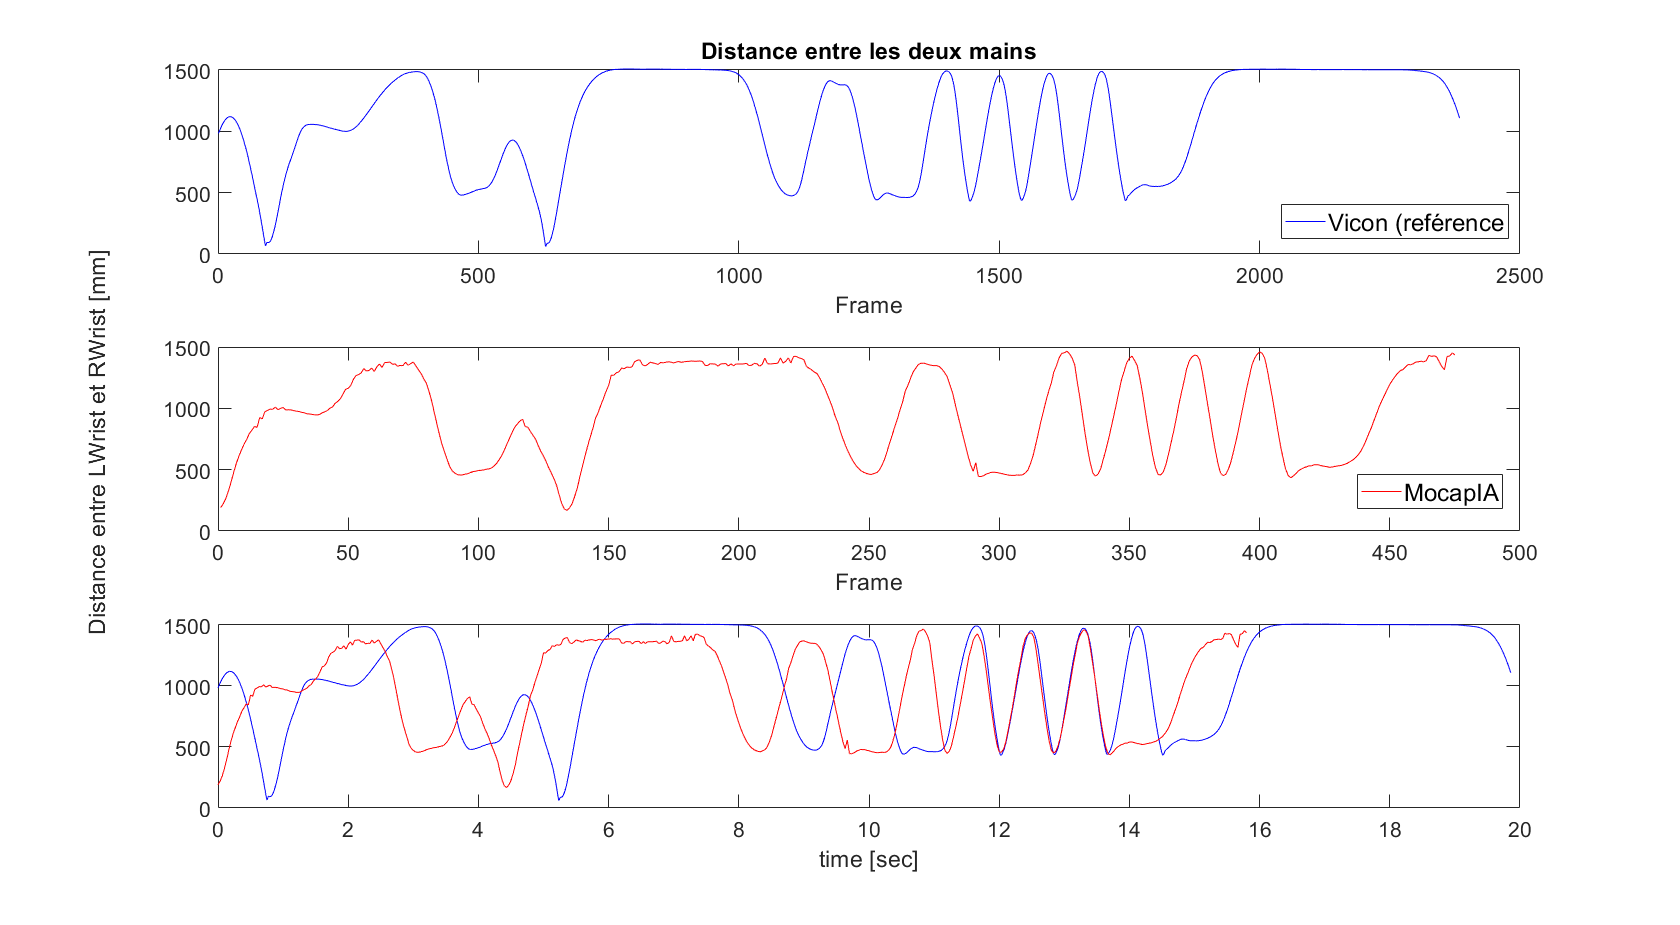
\includegraphics[width=\linewidth]{assets/Capture d'écran process/TX_ViconVSMocapIA/before_sync.png}
        \caption{Avant synchronisation}
        \label{fig:before_sync}
    \end{subfigure}
    
    % On met la légende principale ici (ou sur la 2ème partie, au choix)
    \caption{Synchronisation des données Vicon et MoCapIA (début)}
    \label{fig:sync}
\end{figure}

\begin{figure}[H]
    \ContinuedFloat
    \centering
    % Deuxième sous-figure
    \begin{subfigure}{\textwidth}
        \centering
        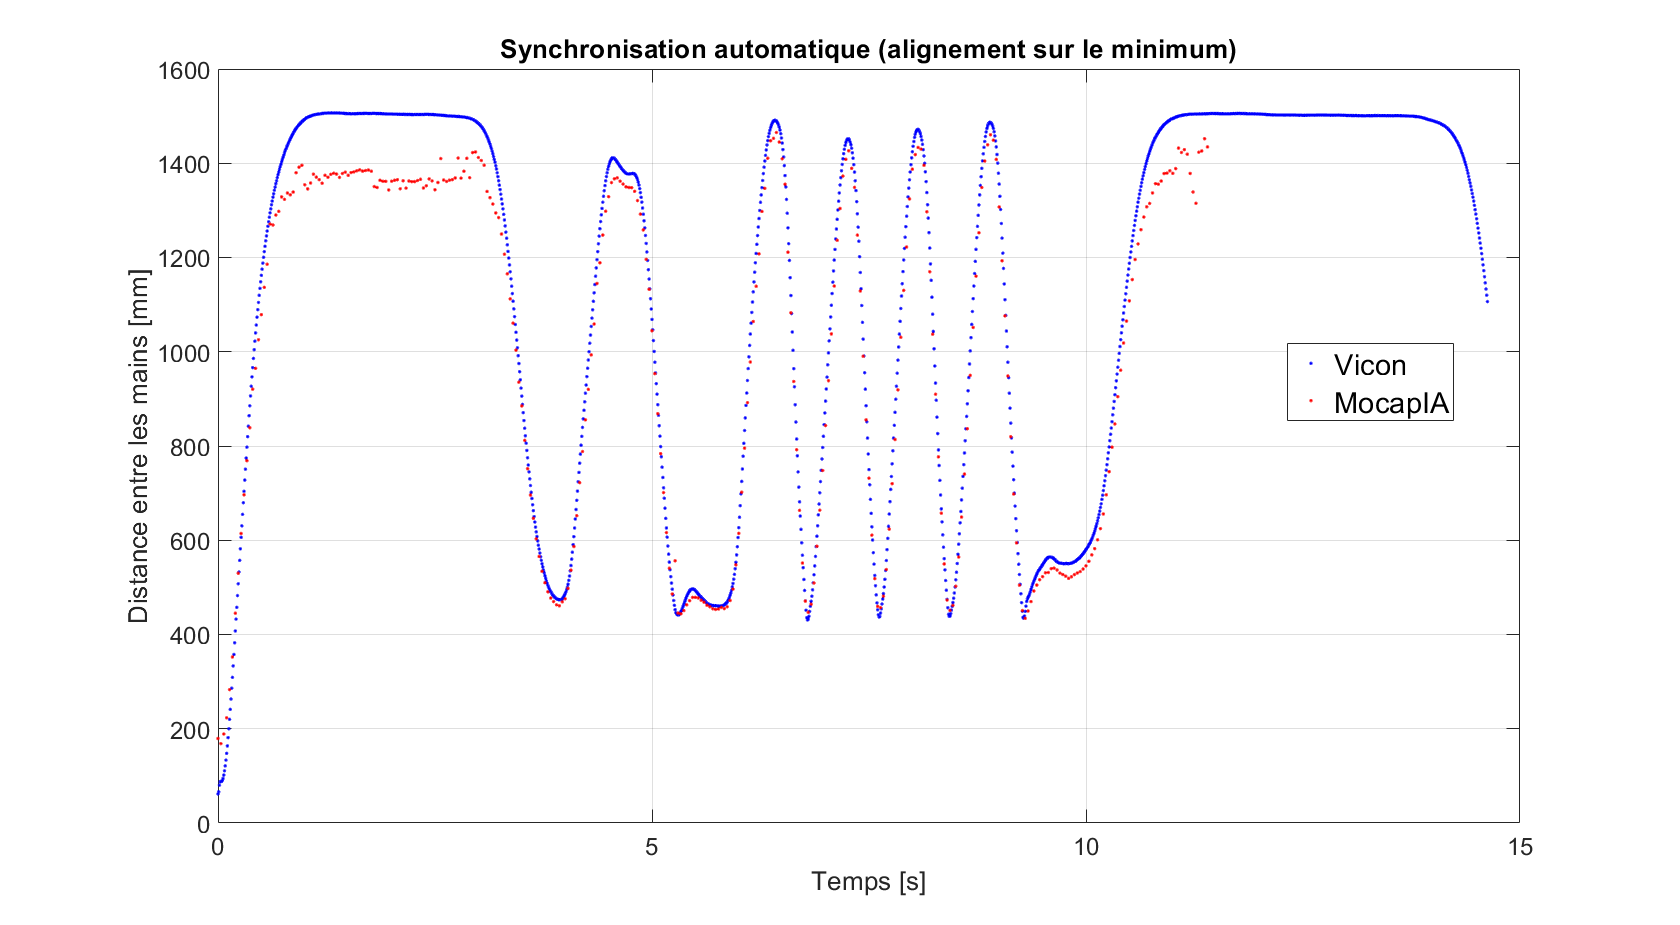
\includegraphics[width=\linewidth]{assets/Capture d'écran process/TX_ViconVSMocapIA/sync.png}
        \caption{Synchronisation appliquée}
        \label{fig:after_sync}
    \end{subfigure}
    
    \caption{Synchronisation des données Vicon et MoCapIA (suite)}
\end{figure}
    
    Ensuite pour chaque articulation notée de 1 à 21, il est nécessaire de calculer déjà l'écart entre les deux systèmes sur l'ensemble des frames. Un "offset" est obligatoirement présent, car les deux systèmes ne placent pas les points caractéristiques exactement au même endroit (ex : le marqueur physique de l'épaule du système Vicon est placée plus en arrière que le marqueur virtuel de l'épaule du système MoCapIA). Pour connaître la précision de notre système par rapport à celui du Vicon, il a été décidé d'ignorer l'offset afin de se concentrer sur la variation des mesures. Ainsi, pour chaque articulation, on calcule la moyenne et l'écart type des erreurs entre les deux systèmes (voir figure \ref{fig:mean_sd_vicon_mocapia}). Ici la moyenne n'a pas vraiment de sens, car elle correspond à l'offset en moyenne au cours du temps. Pour la tête (indice n°13), l'offset est conséquent, parce que le point caractéristique du MoCapIA est situé sur le haut du crâne tandis que le Vicon place le point au centre de la tête, soit un écart de $20cm$. Pour autant des différences sont à noter suivant l'articulation examinée. Les écarts types varient de $8mm$ pour des articulations comme les épaules à $34mm$ pour des points comme la tête ou les poignets. La moyenne des écarts types sur l'ensemble des articulations est de $15.6mm$, autrement dit environ $68\%$ varient dans l'intervalle $[ \text{offset} -15.6mm ; \text{offset} +15.6mm ]$. 
    \begin{figure}[H]
        \centering
        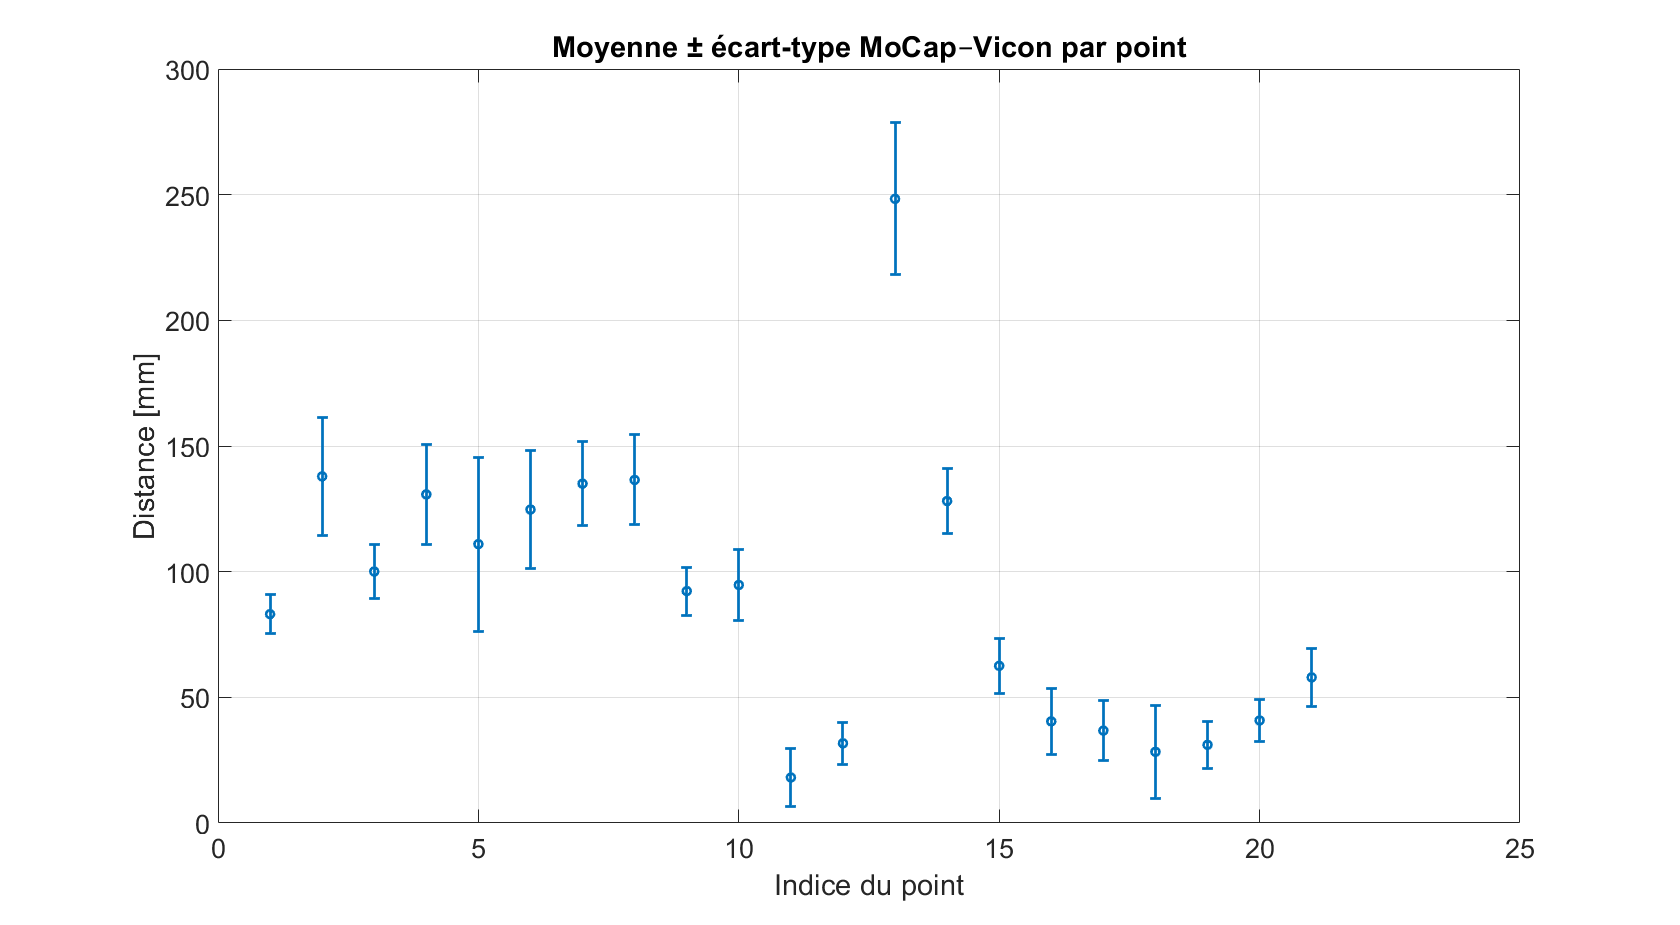
\includegraphics[width=\textwidth]{assets/Capture d'écran process/TX_ViconVSMocapIA/mean_sd_result.png}
        \caption{Moyenne et écart type des erreurs entre Vicon et MoCapIA pour les 21 articulations}
        \label{fig:mean_sd_vicon_mocapia}
    \end{figure}

    Il est intéressant d'utiliser les boxplots (figure \ref{fig:boxplot_vicon_mocapia}) afin de mettre en avant la plage de variation des erreurs (plus représentatif de la stabilité ou non du système que l'écart type). La majorité des mesures, représentée par l'étendue des moustaches (1,5 × écart interquartile), se situe dans une plage de fonctionnement de $57.40 mm$ en moyenne. Cette méthode exclut les valeurs aberrantes, mais restent fidèles au fonctionnement global du système. Même si cette valeur moyenne semble assez faible donc satisfaisante, certaines articulations présentent des plages de variations bien plus importantes. On observe deux situations. La première se trouve au niveau des articulations sensibles du haut du corps, comme les poignets et la tête avec respectivement une variation de $143mm$, $114mm$ et $127mm$. Pour le bas du corps, notamment pour les orteils et le talon, la plage de fonctionnement est bien plus petite ($\approx 30mm$) mais le nombre de valeurs aberrantes est bien plus important en représentant en moyenne $15\%$ des valeurs totales. Au contraire, pour les articulations du haut du corps, on obtient une plage de fonctionnement bien plus grande ($\approx 80mm$) mais avec un pourcentage de valeurs aberrantes inférieures $0 \text{ à } 2\%$ sur l'ensemble des valeurs \cite{OpticalMoCapLongo}.
    \begin{figure}[H]
        \centering
        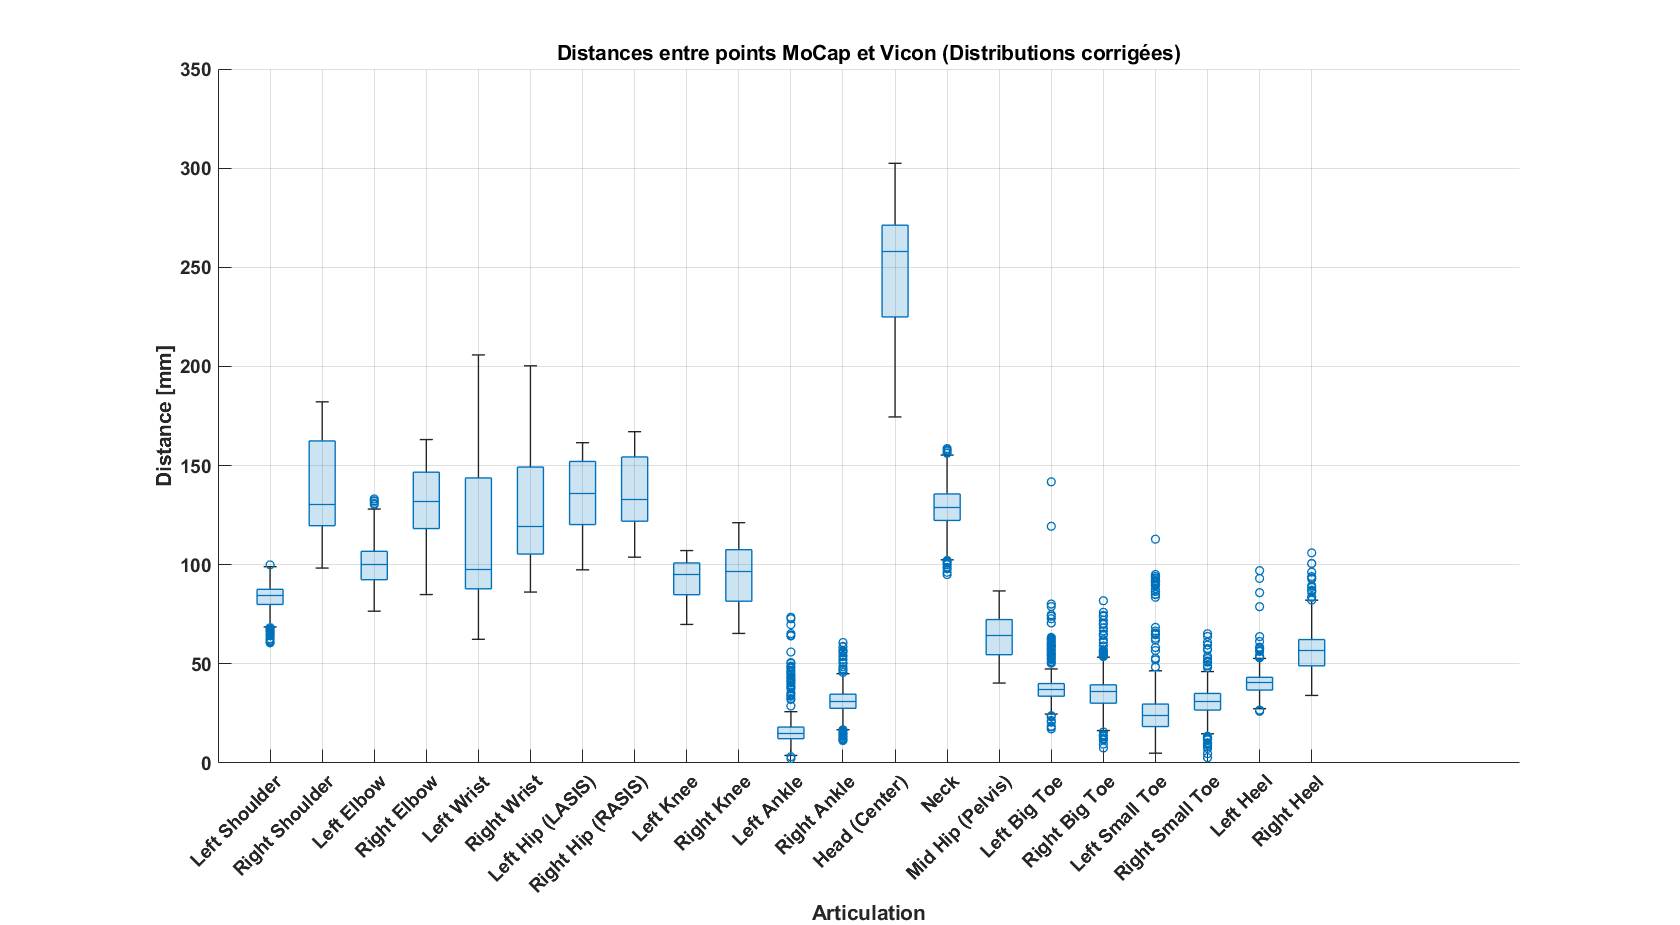
\includegraphics[width=\textwidth]{assets/Capture d'écran process/TX_ViconVSMocapIA/boxplot_vicon_mocap.png}
        \caption{Boxplots des erreurs entre Vicon et MoCapIA pour chaque articulation}
        \label{fig:boxplot_vicon_mocapia}
    \end{figure}

    Il est pertinent d'ajouter l'analyse Bland-Altman afin de comparer la validité de MoCapIA par rapport au système Vicon. Là encore le biais (erreur systématique/constante) représente la différence de positions entre les marqueurs physiques du Vicon et les marqueurs virtuels du modèle utilisé par MoCapIA. La variation aléatoire représente les erreurs réelles de MoCapIA. Les résultats sont bons, avec $\approx 95\%$ des valeurs situées entre $122.2mm$ et $80.2mm$ ($\text{mean} \pm1.96*\text{SD}$).
    \begin{figure}[H]
        \centering
        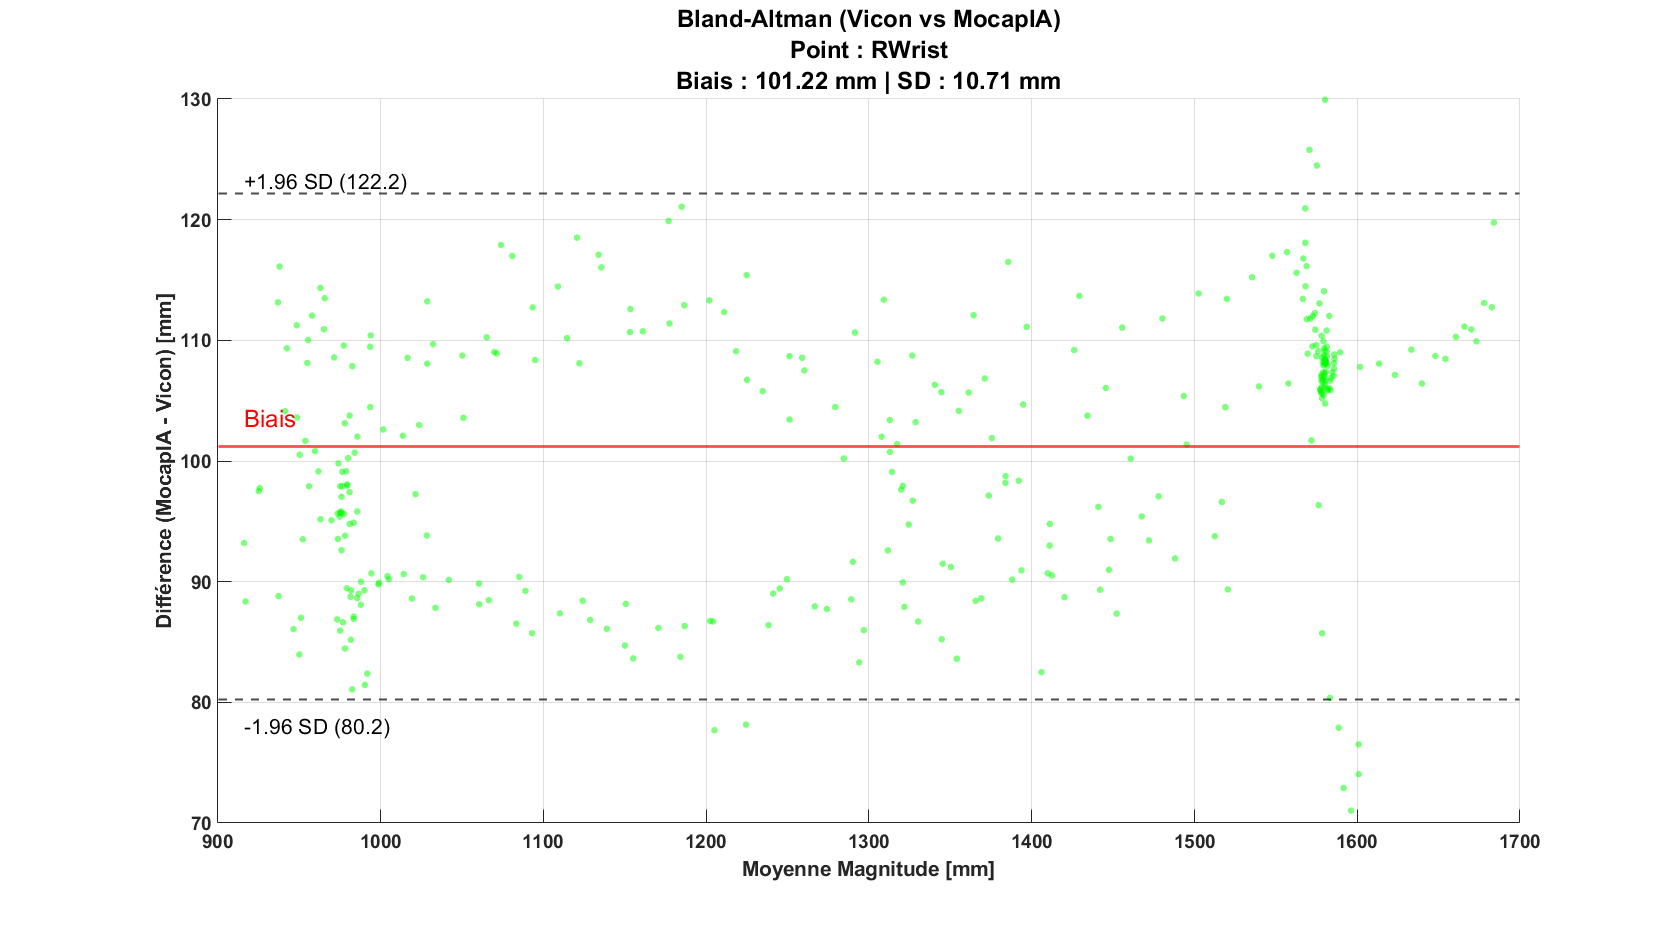
\includegraphics[width=\textwidth]{assets/Capture d'écran process/TX_ViconVSMocapIA/BlandAltman_Vicon_Mocap.png}
        \caption{Analyse Bland-Altman entre Vicon et MoCapIA pour le poignet Droit}
        \label{fig:bland_altman_vicon_mocapia}
    \end{figure} 

    Maintenant que l'analyse de l'erreur de position est faite, il est intéressant d'effectuer une analyse cinématique (angulaire) pour étudier la cohérence biomécanique et l'utilité clinique. Pour ça on utilise le produit scalaire de deux scalaires. Pour trouver l'angle $\theta$ au sommet $B$ formé par les points $A$, $B$ et $C$, on utilise la formule suivante :
    \begin{equation}
        BA \cdot BC = ||BA|| \cdot ||BC|| \cdot \cos(\theta)
    \end{equation}
    Ainsi, on obtient l'angle $\theta$ :
    \begin{equation}
        \theta = \arccos\left(\frac{BA \cdot BC}{||BA|| \cdot ||BC||}\right)
    \end{equation}

    La métrique la plus répandue dans le domaine biomécanique est la RMSE (Root Mean Square Error). En considérant toujours Vicon comme la référence, elle se calcule de cette façon :
    \begin{equation}
        RMSE = \sqrt{\frac{1}{N} \sum_{i=1}^{N} ( \theta_{Vicon}(i) - \theta_{MoCapIA}(i) )^2 }
    \end{equation}
    Avec :
    \begin{description}
        \item[$\theta_{Vicon}(i)$] l'angle mesuré par le système Vicon à la frame $i$
        \item[$\theta_{MoCapIA}(i)$] l'angle mesuré par le système MoCapIA à la frame $i$
        \item[$N$] le nombre total de frames
    \end{description}
    Les résultats montre une bonne performance du système MoCapIA avec une RMSE de $5.28^\circ$ pour le coude gauche et de $2.0^\circ$ pour le genou gauche. Les résultats sont satisfaisants, étant donné que d'après la littérature, les meilleurs résultats obtenus avec des systèmes markerless atteignent une RMSE d'environ $3.5^\circ$ pour des mouvements simples \cite{LSTM}. 

    \begin{figure}[H]
        \centering
        
\includegraphics[width=\textwidth]{assets/Capture d'écran process/TX_ViconVSMocapIA/angle_CoudeG.png}
        \caption{RMSE de l'angle du coude gauche entre Vicon et MoCapIA}
        \label{fig:angle_coudeG}
    \end{figure}

    D'autres résultats secondaires ont été obtenus durant ce test, et sont présentés en Annexe \ref{AnnexVicon_Mocap}.

    En conclusion, l'estimation 2D engendre la majeure partie des erreurs totales du système avec des autres de grandeurs atteignant la dizaine de centimètres pour certaines articulations. La calibration et la triangulation n'engendrent que très peu d'erreurs à comparer, avec des erreurs moyennes de l'ordre du centimètre. Les erreurs de ces modèles d'IA open-source comme celui utilisé (RTMPose) comportent des erreurs à la fois à cause des données d'entraînement pas totalement adaptées à la biomécanique et des problèmes d'occultation durant l'entraînement \cite{MarkerlessforBiomecha}. D'un autre côté, il est pourtant important de notifier que la précision angulaire de MoCapIA est satisfaisante par rapport à sa précision de position. C'est donc sur ce premier point que la suite des réalisations va se concentrer.

\section{Amélioration du processus MoCapIA}

    À ce stade du stage, l'estimation 2D est identifiée comme la principale source d'erreurs du système MoCapIA. Ces erreurs empêchent une analyse biomécanique sérieuse et fiable. De plus le problème auquel il faut faire face est le suivant : \textbf{RTMPose} (modèle de détection des articulations) est le modèle OpenSource \textbf{le plus précis actuellement disponible} pour une estimation 2D du corps humain assez rapide \cite{HumanPoseEstimationModels}\cite{RTMPose}. Les solutions open-source souffrent de négligence durant l'entraînement, c'est de là que viennent les erreurs importantes \cite{MarkerlessforBiomecha}. Il est donc nécessaire d'ajouter des étapes supplémentaires au processus MoCapIA pour corriger les erreurs restantes.

    Après plusieurs recherches, un module OpenSource appelé \textbf{Pose2Sim} a été trouvé. Ce module reprend en partie le processus MoCapIA mais ajoute des étapes supplémentaires conçues pour l'analyse biomécanique. En effet, en plus d'effectuer une calibration, une estimation 2D et une reconstruction 3D simple, Pose2Sim ajoute un processus de filtrage, une augmentation du nombre de marqueurs ainsi qu'une correction biomécanique des mouvements. L'ajout de marqueurs virtuels permettrait d'utiliser ce package \textit{opensim} et le logiciel OpenSim, qui pourront eux-mêmes corriger les erreurs restantes après le filtrage et apporter les informations manquantes pour une analyse plus poussée. Ce module utilise d'ailleurs \textbf{RTMLib} pour la détection des points caractéristiques, qui appartient à la même famille que \textbf{RTMPose} (le modèle utilisé par MoCapIA).
    \begin{figure}[H]
        \centering
        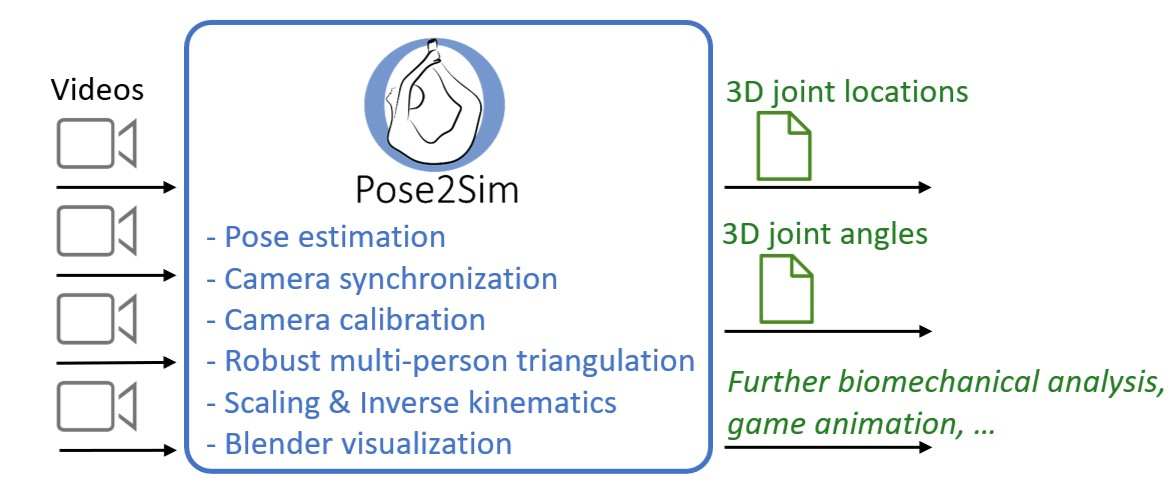
\includegraphics[width=0.8\linewidth]{assets/Capture d'écran process/Pose2Sim/Pose2Sim_workflow.jpg}
        \caption{Processus Pose2Sim (source : \href{https://github.com/perfanalytics/pose2sim}{GitHub Pose2Sim})}
        \label{fig:pose2sim_workflow}
    \end{figure}
    
    Mais avant d'implémenter ces nouvelles étapes, il est important de comparer les étapes communes entre MoCapIA et Pose2Sim (calibration, estimation 2D et triangulation) pour s'assurer de garder la version la plus précise. Pour ça, on compare les longueurs des membres du corps sur l'ensemble du mouvement. La stabilité fait aussi partie des paramètres qui seront analysés. En comparant les deux fichiers .csv de points 3D, on peut ainsi calculer sur l'ensemble du mouvement la longueur de chaque membre du corps. Sur la figure \ref{fig:boxplot_p2s_mocap}, la stabilité moyenne de Pose2Sim est supérieur, ce qui s'explique par le fait que les données de Pose2Sim dispose d'un filtrage. D'ailleurs le nombre d'outliers est plus important pour le système MoCapIA.
    \FloatBarrier
    \begin{figure}[H]
        \centering
        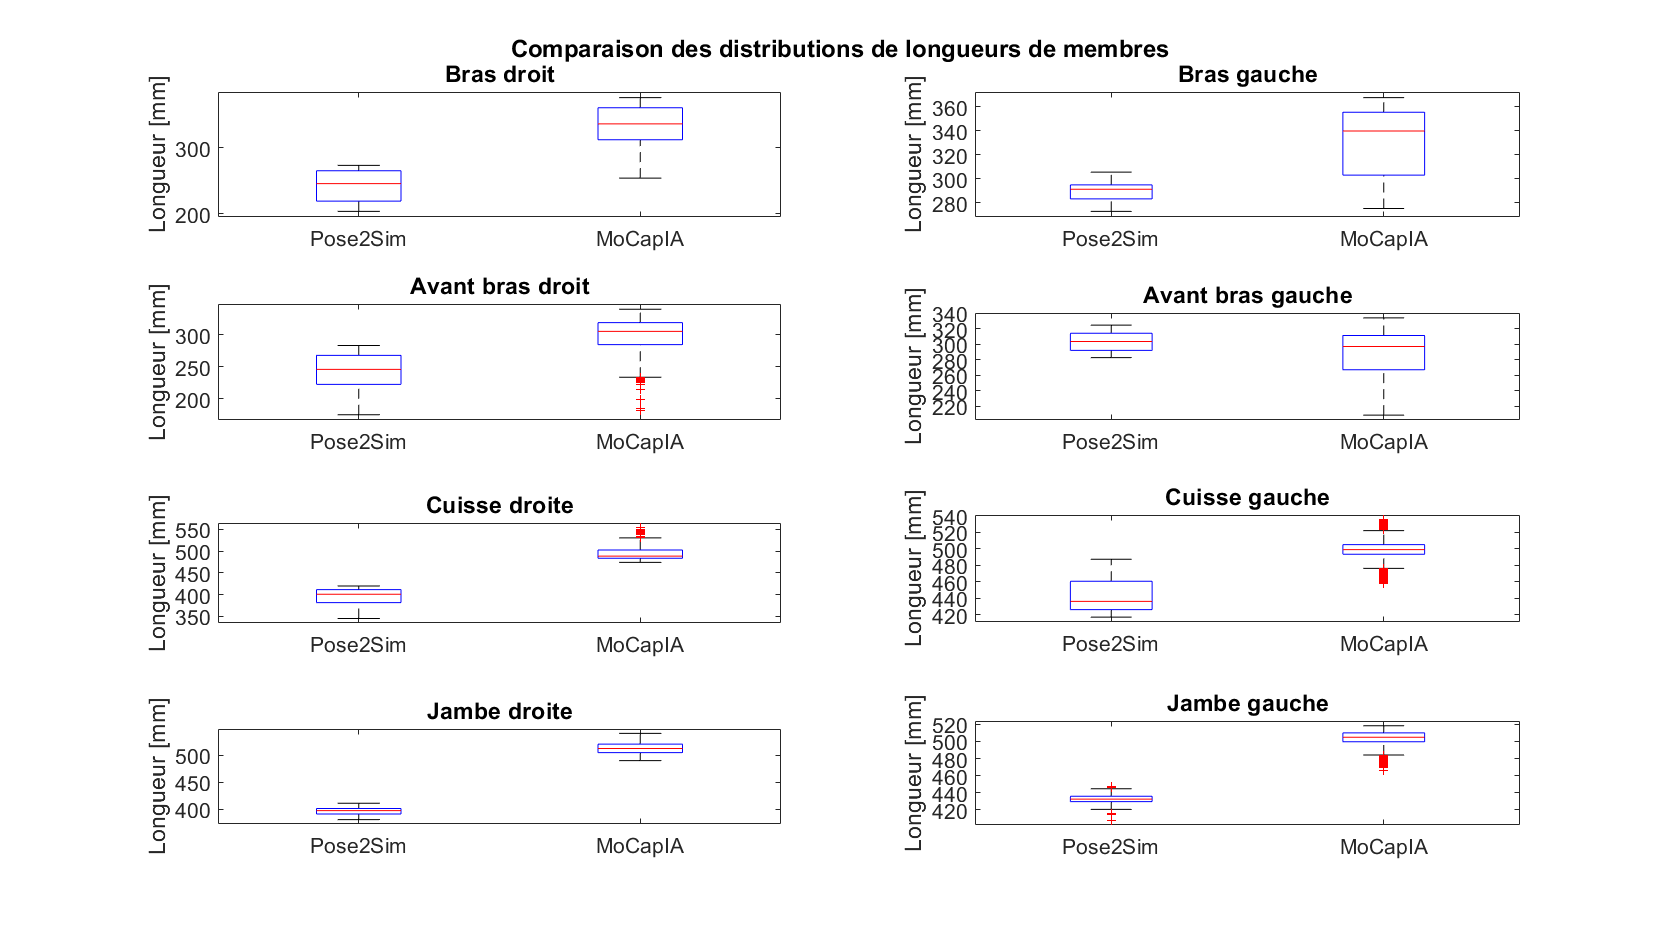
\includegraphics[width=\linewidth]{assets/Capture d'écran process/Pose2Sim/boxplot_P2S_Mocap.png}
        \caption{Comparaison des distributions de la longueur des membres entre Pose2Sim et MoCapIA}
        \label{fig:boxplot_p2s_mocap}
    \end{figure}
    
    \FloatBarrier
    D'un autre côté, les deux systèmes utilisent le même modèle de squelette (Halpe26 : figure \ref{fig:halpe26}) ; il est donc possible, à l'aide des longueurs théoriques mesurées sur le sujet, de comparer la précision des deux systèmes. 
    
    \begin{table}[h!]
    \centering
    \renewcommand{\arraystretch}{1.5}
    \begin{tabularx}{\textwidth}{|l|>{\centering\arraybackslash}X|>{\centering\arraybackslash}X|>{\centering\arraybackslash}X|} 
        \hline
         & \textbf{Longueur bras gauche} & \textbf{Longueur bras droit} & \textbf{Erreur moyenne (ensemble)}\\
        \hline
        Mesure théorique & $290mm$ & $290mm$ & x \\
        \hline
        Moyenne Pose2Sim & $288.37mm$ & $243.80mm$ & $44.4mm$ \\
        \hline
        Moyenne MoCapIA & $301.46mm$ & $284.90mm$ & $23.3mm$ \\
        \hline
    \end{tabularx}
    \caption{Comparaison des différents systèmes de caméras}
    \label{tab:cameras}
\end{table}

    Finalement l'erreur moyenne des membres par rapport aux valeurs théoriques du  processus MoCapIA est inférieur à celle de Pose2Sim. C'est donc ce pipeline qui sera conservé pour la suite du projet. Pour autant, il est nécessaire de filtrer nos valeurs et d'ajouter les étapes suivantes (augmentation de marqueurs et correction biomécanique) qui vont être testées et implémentées ci-dessous.

\section{Implémentation du filtrage}

    Même si Pose2Sim n'est pas aussi juste que MoCapIA sur la construction d'un modèle 3D simple, la figure \ref{fig:boxplot_p2s_mocap} montre que MoCapIA obtient plus de valeurs aberrantes (croix rouges sur le graphique). Pour réduire ces erreurs, il est possible d'implémenter des filtres sur les données 3D. Plusieurs types de filtres sont disponibles dans le package Pose2Sim. Il a donc été décidé de tous les tester pour déterminer lequel est le plus adapté aux données biomécaniques issues de MoCapIA. Les filtres testés sont les suivants :
    \begin{itemize}
        \item Filtre LOESS
        \item Filtre Gaussian
        \item Filtre GCV Spline
        \item Filtre Butterworth Speed
        \item Filtre Kalman
        \item Filtre Butterworth Classique
        \item Filtre Hampel
    \end{itemize}
    Les 2 derniers filtres sont ceux qui ont été garder après leur étude (les autres résultats sont présentés en Annexe \ref{Annexfiltres}). En effet, les autres ne sont pas adaptés aux signaux biomécanique à l'inverse du filtre Butterworth \cite{FiltresComparaison}\cite{Butter}\cite{Butter2}. Le filtre \textit{Hampel} est un filtre de détection de valeurs aberrantes qui a été ajouté en amont des autres filtres pour améliorer leur efficacité. Voici son impact sur l'articulation LWrist (poignet gauche), l'une des articulations la plus sujette aux erreurs :
    \begin{figure}[H]
        \centering
        \begin{subfigure}{\textwidth}
            \centering
            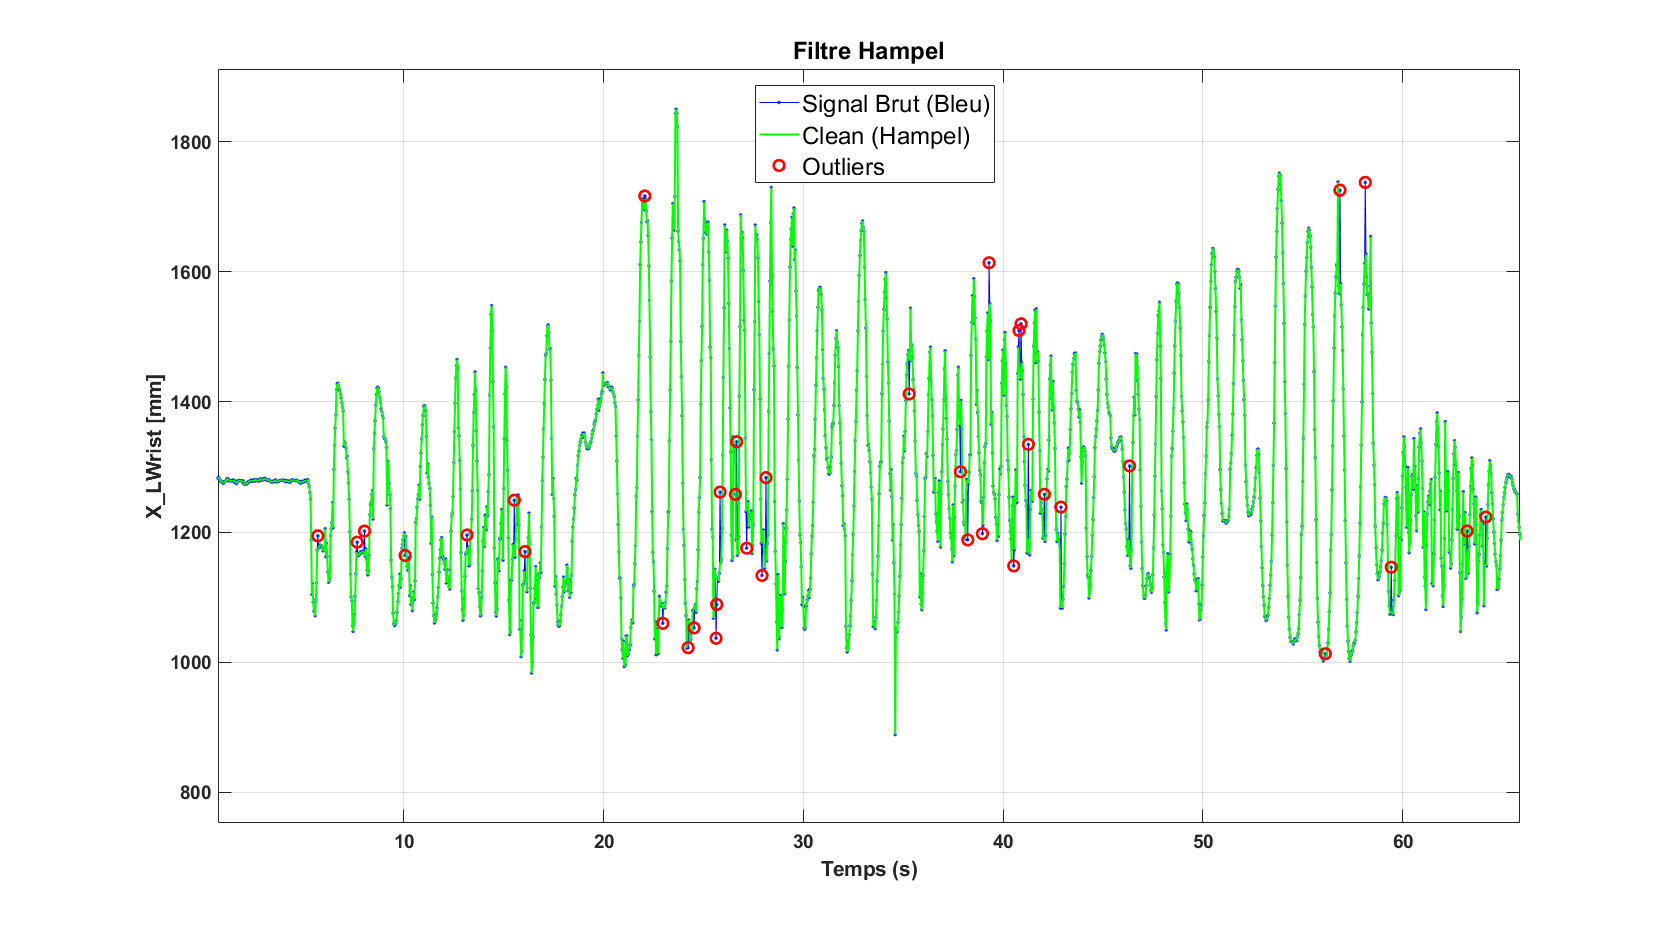
\includegraphics[width=\textwidth]{assets/Capture d'écran process/Tests Filtres 3D/valid/hampel.png}
            \caption{Filtrage Hampel appliqué}
            \label{fig:filtre_hampel}
        \end{subfigure}
        \hfill
        \begin{subfigure}{\textwidth}
            \centering
            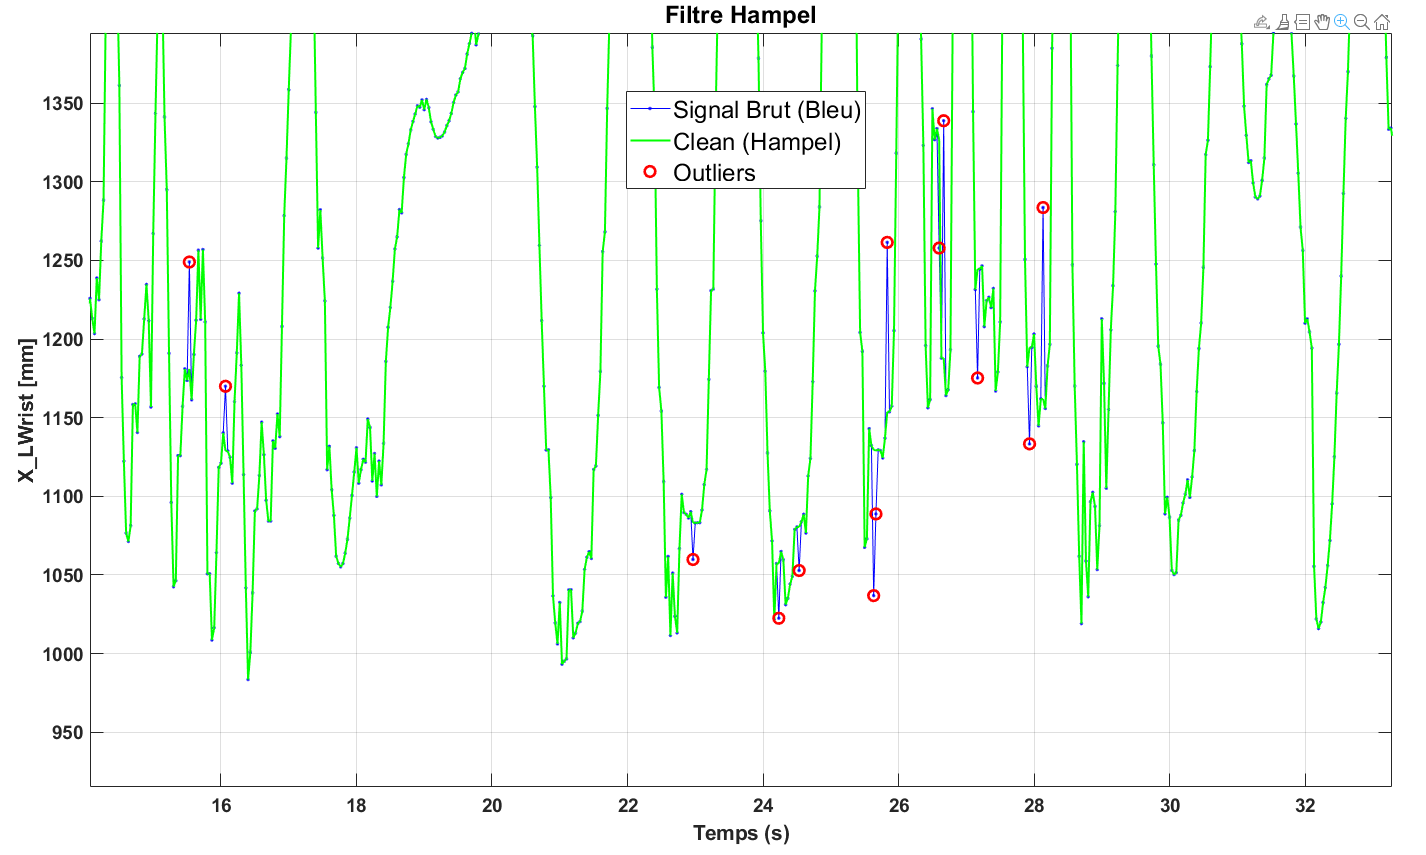
\includegraphics[width=0.8\textwidth]{assets/Capture d'écran process/Tests Filtres 3D/valid/hampel_zoom.png}
            \caption{Zoom sur l'action du filtre Hampel}
            \label{fig:filtre_hampel_zoom}
        \end{subfigure}
        \caption{Impact du filtre Hampel sur le signal du poignet gauche}
        \label{fig:filtre_hampel_total}
    \end{figure}

    Une fois les valeurs aberrantes supprimées, les autres filtres sont appliqués. Le filtre butterworth est un filtre numérique récursif très répandu dans le domaine biomécanique grâce à la simplicité de son écriture mathématique et de calcul. Il dépend du choix de la fréquence de coupure $f_c$ et de l'ordre $n$. La fréquence typique choisie pour le filtrage des signaux biomécaniques est de $f_c = 6$ à $10 Hz$ et l'ordre est souvent compris entre $2$ et $4$ \cite{Biblio_Filtrage1990}\cite{Butter}\cite{Butter2}. C'est celui qui a été intégré au processus.

    \begin{figure}[H]
        \centering
        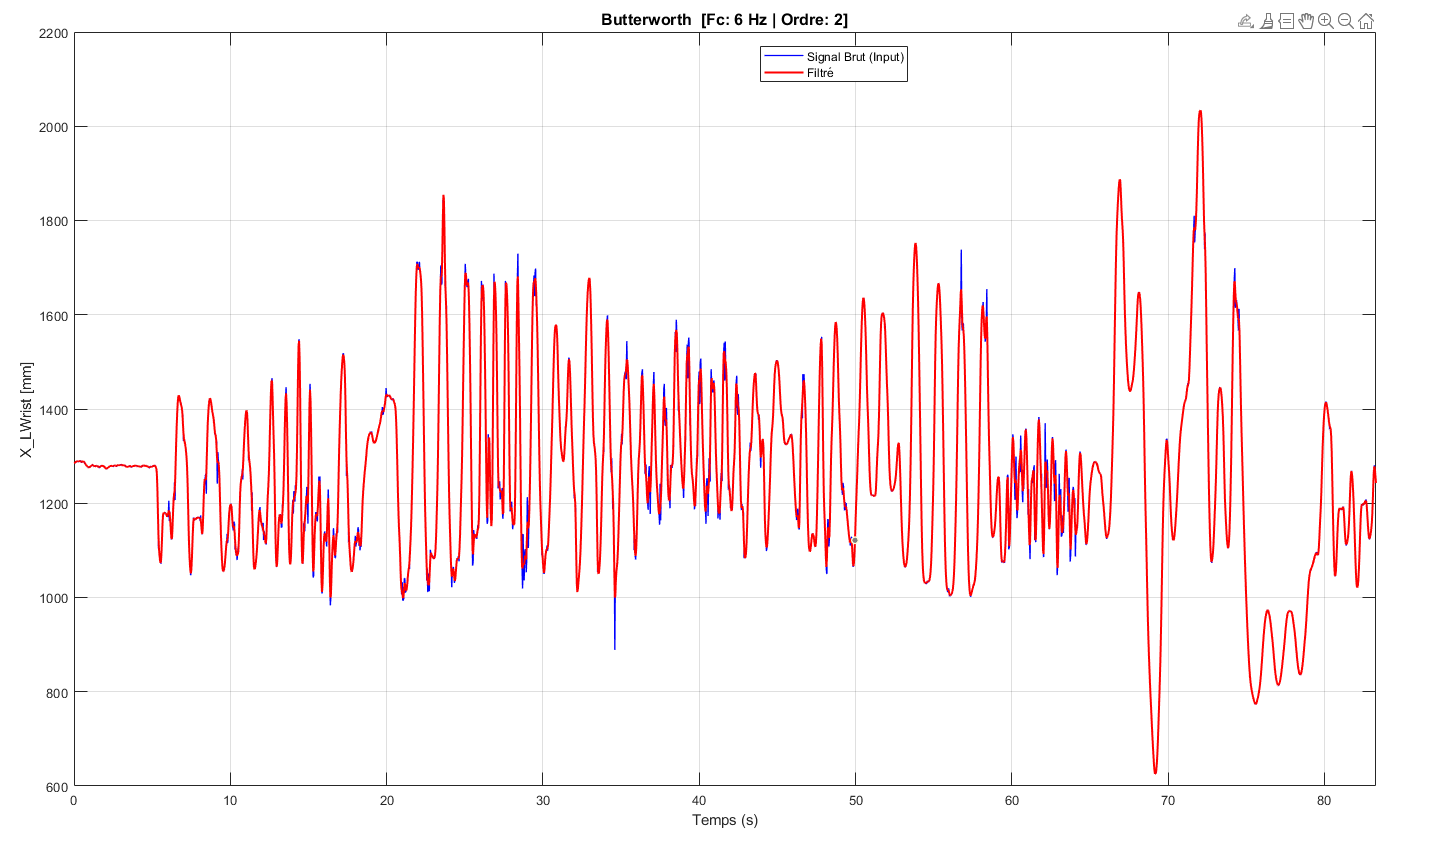
\includegraphics[width=\textwidth]{assets/Capture d'écran process/Tests Filtres 3D/valid/butterworth.png}
        \caption{Impact du filtre Butterworth sur le signal du poignet gauche}
        \label{fig:filtre_butterworth}
    \end{figure}
    Sur la figure ci-dessus, il n'est pas facile de valider le filtre. Pour ça, on applique la méthode de Bland-Altman qui permet de comparer deux séries de données. En comparant les données brutes et les données filtrées, on observe que la majorité des points ($\approx 95\%$) se situent dans les limites de concordance ($\text{mean} \pm1.96*\text{SD}$) ce qui valide l'efficacité du filtre.
    \begin{figure}[H]
        \centering
        
\includegraphics[width=\textwidth]{assets/Capture d'écran process/Tests Filtres 3D/valid/Bland_Altman_butterworth.png}
        \caption{Analyse de Bland-Altman entre les données brutes et les données filtrées sur la coordonnée X du poignet gauche}
        \label{fig:bland_altman_butterworth}
    \end{figure}

\section{Implémentation de l'augmentation de marqueurs}

    Avec le modèle de marqueur Halpe26, on a seulement 26 marqueurs. Ce n'est pas suffisant pour mener une étude du mouvement complète. On a donc besoin d'augmenter ce nombre de marqueurs. Il existe d'autres types de squelettes avec plus de marqueurs, mais leurs fiabilités laisse à désirer. On se penche donc sur une technique d'\textit{augmentation de marqueurs (marker augmentation)} qui consiste à utiliser un modèle d'apprentissage profond. Par l'intermédiaire d'un réseau \textit{Long Short-Term Memory (LSTM)} entraîné pour la capture la dynamique temporelle des données de mouvement, il est possible de transformer 20 keypoints provenant du modèle simpliste en un ensemble de \textbf{43 marqueurs atomiques} (voir figures \ref{fig:lstm_augmentation}, \ref{fig:halpe26_markers} et \ref{fig:lstm_markers}). 
    
    \begin{figure}[H]
        \centering
        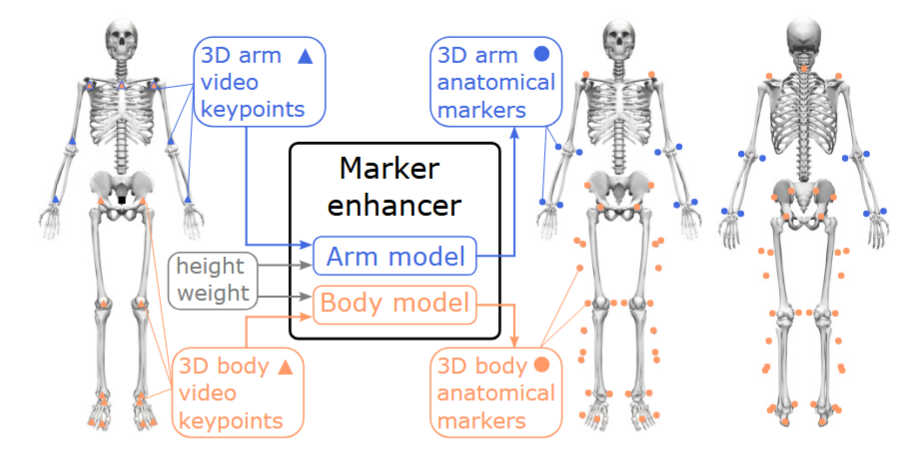
\includegraphics[width=0.8\textwidth]{assets/Capture d'écran process/Halpe26vsLSTM/LSTM.png}
        \caption{L'augmentation de marqueurs à l'aide d'un réseau LSTM (cf. \cite{LSTM})}
        \label{fig:lstm_augmentation}
    \end{figure}

    Cela est rendu possible grâce une architecture qui intègre une mémoire à long terme qui permet de conserver les informations intéressantes durant un certain temps. Contrairement aux réseaux de neurones classiques, les LSTM sont donc capables de lier les informations passées au contexte actuel. Cela permet de prédire des trajectoires fluides et cohérentes pour les nouveaux marqueurs \cite{UnderstandingLSTM}.
    \begin{figure}[H]
        \centering
        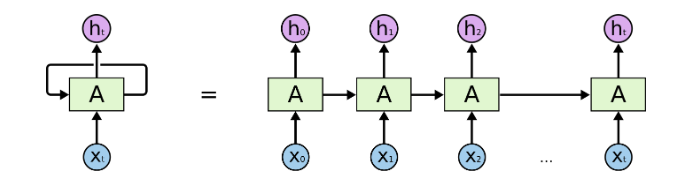
\includegraphics[width=0.8\textwidth]{assets/Capture d'écran process/Halpe26vsLSTM/LSTM_neurones.png}
        \caption{Architecture du réseau récurrent LSTM pour l'augmentation de marqueurs (cf. \cite{UnderstandingLSTM})}
        \label{fig:lstm_architecture}
    \end{figure}

    Cette technique a été implémentée à la suite du filtrage. Sur des mouvements de référence (marche, squat), l'impact de l'augmentation de marqueurs est faible, mais permet tout de même de passer d'une erreur cinématique moyenne (RMSE) de $9.6^\circ$ à $4.1^\circ$ pour les degrés de liberté rotationnels \cite{LSTM}. L'avantage majeur de l'augmentation de marqueurs est d'avoir une meilleure représentation des segments du corps humain et ainsi capturer les mouvements de rotation du bras sur lui-même par exemple. C'est donc sur les mouvements plus complexes (ex : pompes, rouler au sol) que l'augmentation de marqueurs montre tout son intérêt. En conservant une erreur moyenne de $4.1^\circ$, il surpasse largement la performance du modèle précédent (Halpe26 seul) qui atteint une erreur moyenne de $40.4^\circ$. En effet, certaines rotations ne peuvent pas être correctement estimées avec des articulations représentées seulement par un seul marqueur. 
    \begin{figure}[H]
    \centering

    \begin{subfigure}{0.48\textwidth}
        \centering
        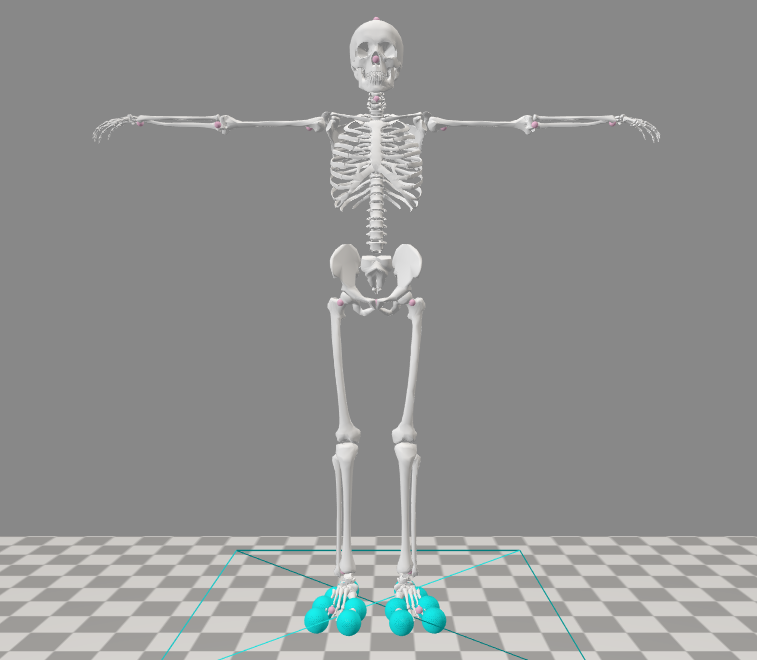
\includegraphics[width=\linewidth]{assets/Capture d'écran process/OpenSim/markerHALPE26.png}
        \caption{Squelette avec les marqueurs Halpe26}
        \label{fig:halpe26_markers}
    \end{subfigure}
    \hfill
    \begin{subfigure}{0.51\textwidth}
        \centering
        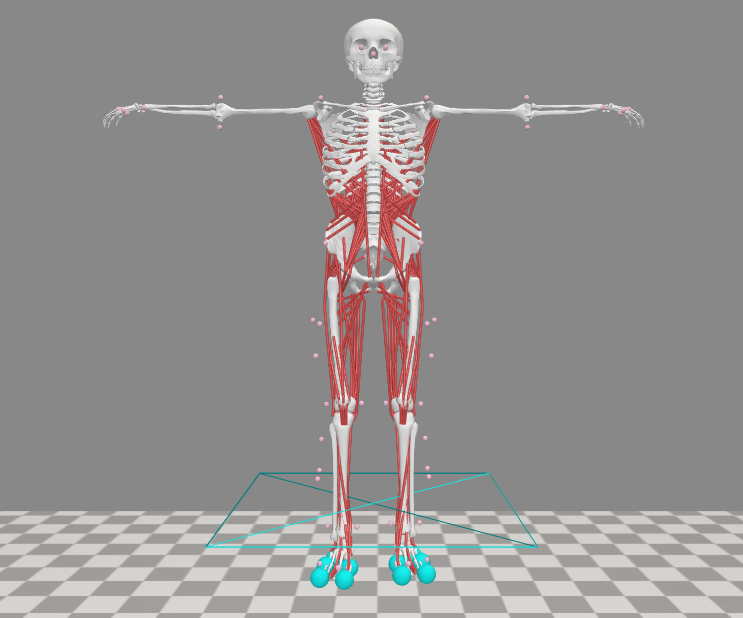
\includegraphics[width=\linewidth]{assets/Capture d'écran process/OpenSim/markeraugmented.png}
        \caption{Squelette avec l'augmentation de marqueurs}
        \label{fig:lstm_markers}
    \end{subfigure}
    
    \caption{Comparaison du squelette avant et après l'augmentation de marqueurs sur OpenSim}
    \label{fig:comparaison_marqueurs}
    \end{figure}

\section{Intégration de la correction biomécanique}
    Avec les nouveaux fichiers contenant les nouveaux marqueurs et le package \textit{opensim}, il est possible d'ajouter deux étapes de correction biomécanique.  Nous avons décomposé cette étape en deux objectifs cruciaux : le \textit{Scaling} (la mise à l'échelle) et le \textit{Kinematic Fitting} (l'ajustement cinématique).

    \subsection{\textit{\textbf{Scaling}}}
        Le \textit{\textbf{Scaling}} consiste à adapter un modèle générique d'un squelette aux dimensions de notre sujet. Cette étape est essentielle avant d'exécuter l'analyse cinématique, car chaque individu possède des proportions biomécaniques différentes. On utilise donc ce modèle $.osim$ ainsi que nos coordonnées 3D (fichier $.trc$) d'un essai statique (T-Pose). En mesurant les distances entre des paires de marqueurs (ex : \texttt{r\_knee} et \texttt{r\_ankle}), on obtient les facteurs d'échelle de chaque membre du corps.
        \begin{equation}
            fe = \frac{d_{marqueurs}}{d_{generique}}
        \end{equation}
        \begin{description}
            \item[$fe$] le facteur d'échelle
            \item[$d_{marqueurs}$] la distance mesurée entre les marqueurs de chaque membre du sujet
            \item[$d_{generique}$] la distance entre les mêmes marqueurs sur le modèle générique
        \end{description}
        Ces facteurs d'échelles vont permettre d'ajuster le modèle $.osim$ initial aux dimensions du sujet. De plus, en prenant en compte la masse du sujet donnée dans la configuration, on peut ajuster les propriétés inertielles du modèle (masse, centre de masse, moments d'inertie) en fonction des proportions du sujet. Finalement, on obtient un nouveau modèle $.osim$ avec les propriétés biomécaniques du sujet.

    \subsection{\textit{\textbf{Cinématique Inversée}}}
    La \textit{\textbf{Cinématique Inversée} (Inverse Kinematics - IK)} permet de contraindre les données à un modèle musculosquelettique, garantissant ainsi la cohérence biomécanique des mouvements. Autrement dit, on ajoute des contraintes sur les résultats obtenus précédemment et on essaie de minimiser les erreurs pour satisfaire au mieux ces contraintes. Son utilisation est reconnue dans la littérature scientifique de biomécanique \cite{LSTM}\cite{Butter2}. On va donc utiliser le modèle $.osim$ mis à l'échelle ainsi que les coordonnées 3D (fichier $.trc$) du mouvement. L'algorithme calcule de nouvelles positions pour chaque marqueur à différend angles. Cet ensemble d'angles $q$ est censé minimiser la somme des carrés des distances entre chaque marqueur expérimentaux. C'est comme ça que les angles articulaires du mouvement sont obtenus. 

    \begin{equation}
        \min_{q} \sum_{i=1}^{n} w_i \| p_{i}^{exp} - p_{i}^{sim}(q) \|^2
    \end{equation}

    \begin{description}
        \item[$w_i$] le poids attribué au marqueur $i$
        \item[$p_{i}^{exp}$] la position expérimentale du marqueur $i$
        \item[$p_{i}^{sim}(q)$] la position simulée du marqueur $i$ en fonction des angles articulaires $q$
        \item[$n$] le nombre total de marqueurs 
    \end{description}

    Les résultats obtenus après l'étape de cinématique inversée montrent une nette amélioration de la cohérence biomécanique des mouvements. En comparant les angles articulaires des marqueurs augmentés et du résultat final après la cinématique inversée et le scaling avec le Vicon, on observe une réduction significative des erreurs par rapport aux données de référence du Vicon. Les données provenant d'OpenSim obtiennent un meilleur résultat avec une RMSE de $5.21^\circ$ contre $7.55^\circ$ pour les données avant OpenSim. La figure \ref{fig:ik_results} illustre cette amélioration sur la flexion du genou droit. 
    \begin{figure}[H]
        \centering
        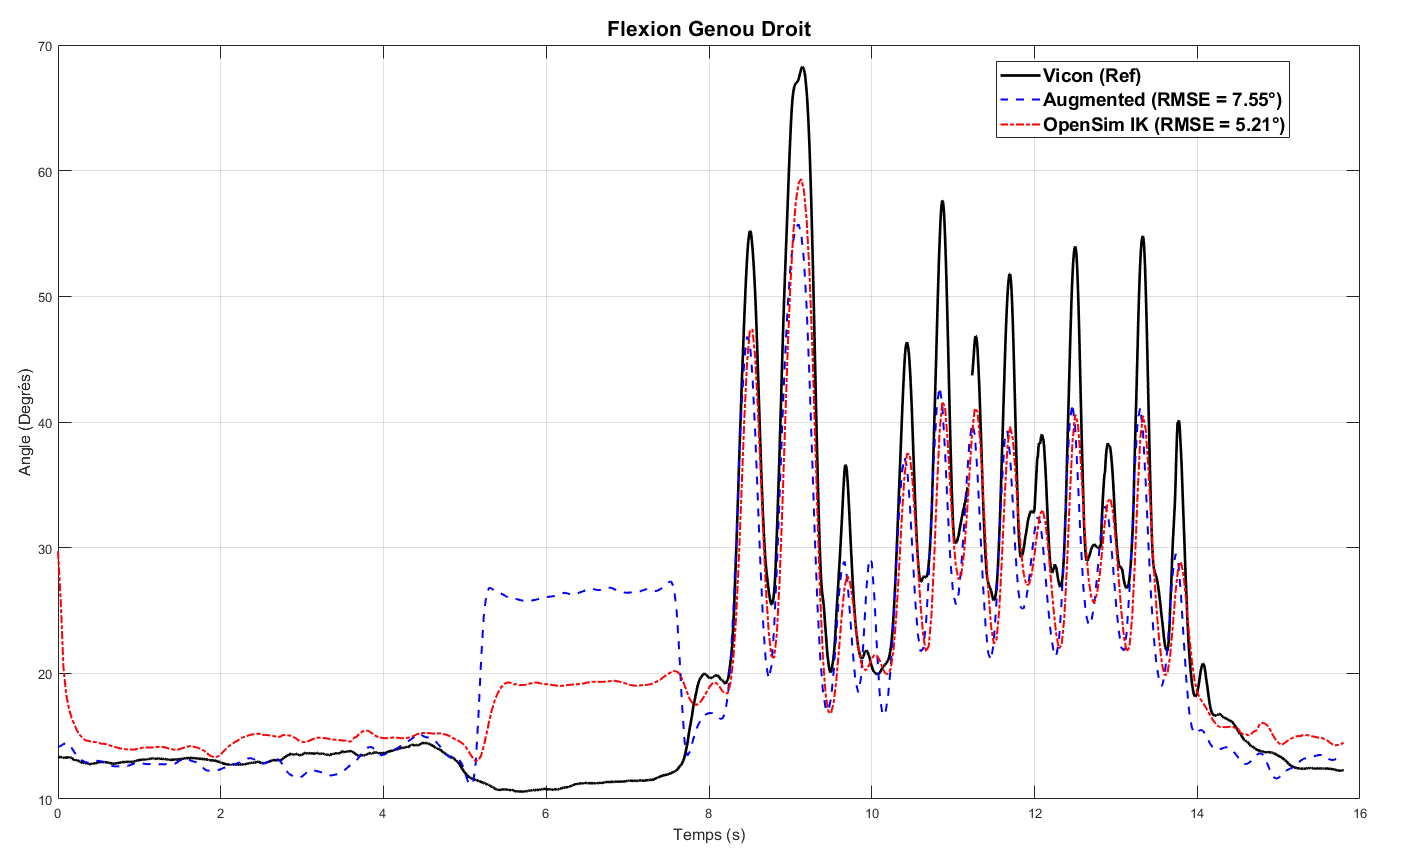
\includegraphics[width=\textwidth]{assets/Capture d'écran process/OpenSim/result.png}
        \caption{Comparaison des angles du genou droit avant et après l'IK d'OpenSim}
        \label{fig:ik_results}
    \end{figure}

    Pour clôturer cette partie, il a été observé que l'ajout des dernières étapes ont permis d'améliorer significativement la qualité des données biomécaniques obtenues avec le système MoCapIA en forçant un squelette humain cohérent sur les données. La $RMSE$ angulaire au début du stage était proche de celle obtenue avec OpenSim mais maintenant la longueur des membres est fixé et donc bien plus cohérente. De plus on dispose désormais de 43 marqueurs au lieu de 26, ce qui permet une analyse plus poussée des mouvements complexes.

\section{Recherche complémentaire : SAM 3D}

Durant le stage, une nouvelle méthode de capture de mouvement markerless a été publiée par Meta AI Research. Appelé \textbf{SAM 3D}, son fonctionnement est bien différent de MoCapIA. Cette technologie est capable de créer un modèle 3D avec seulement une image, un seul point de vue. Autrement dit, la multi-view n'est plus nécessaire ce qui pourrait mener à un gain de temps, de coût et de complexité phénoménal. Sorti en fin novembre 2025, elle pourrait bien révolutionner le domaine de la motion capture sans marqueur. Elle est composée de deux modèles distincts : SAM 3D Object pour les objets et scènes, \textbf{SAM 3D Body} pour les corps humains. C'est ce dernier qui va nous intéresser. Pour déduire une reconstruction 3D à partir d'une seule image, l'Intelligence Artificielle est au cœur de son fonctionnement :
\begin{figure}[H]
    \centering
    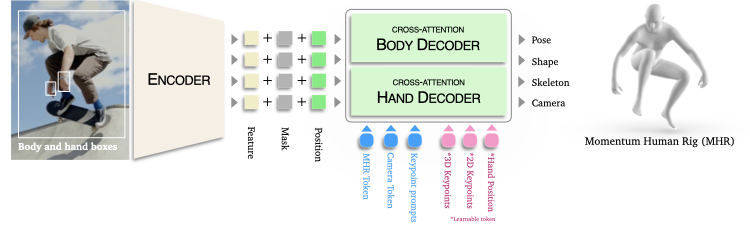
\includegraphics[width=0.8\textwidth]{assets/Capture d'écran process/SAM 3D/SAM3D_workflow.png}
    \caption{Processus SAM 3D Body}
    \label{fig:sam3D_workflow}
\end{figure}

Étant donné que cette technologie est toute récente, peu d'informations sont disponibles sur son fonctionnement interne. De plus, il n'existe pas encore de publication scientifique détaillant ses performances lors de tests rigoureux. Enfin son application est encore limitée à une image. Tel qu'il a été publié, il permet de retourner un modèle 3D à parti d'une image, mais pour l'instant incapable de créer un mouvement au cours du temps en 3D. Ce sont sur ces points que l'équipe a décidé d'approfondir ses recherches durant les dernières semaines du stage.

Disponible en opensource sur GitHub et HuggingFace, le code a été installé localement. En modifiant son code source, il a été possible de lui faire traiter des vidéos. En extrayant chaque frame de la vidéo, on peut ainsi obtenir une séquence de modèles 3D au cours du temps. Pour ça on exécute SAM 3D Body sur chaque frame de la vidéo. Il détecte de la même façon que MoCapIA les points caractéristiques 2D du corps humain à l'aide du modèle Halpe26. Il est donc à première vue possible de comparer ses performances à celle du Vicon et MoCapIA. Pourtant, des problèmes majeurs sont apparus lors de l'utilisation de SAM 3D Body :
\begin{itemize}
    \item Problème de référentiel : À chaque image, le modèle SAM 3D Body est lancé indépendamment. Même si le modèle 3D est centré sur le corps humain, on ne sait pas exactement comment il calcule le référentiel. En conséquence, le modèle 3D se décale dans l'espace au cours du temps.
    \item Problème d'échelle : Le modèle 3D retourné par SAM 3D Body n'est pas à l'échelle réelle. En effet, avec un seul point de vue, il estime la taille du sujet, mais sans aucune référence de distance. Le modèle, même si les coordonnées semblent justes, n'est pas à l'échelle réelle.
    
    \begin{figure}[H]
    \centering

    \begin{subfigure}{0.38
        \textwidth}
        \centering
        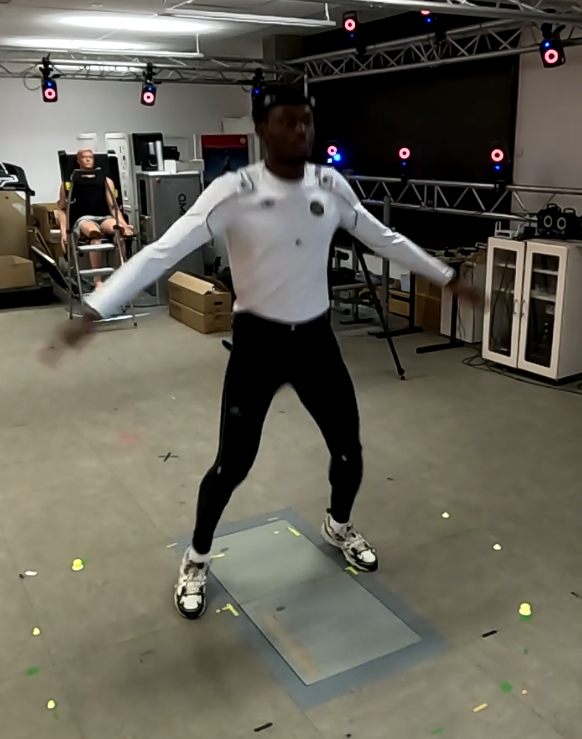
\includegraphics[width=\linewidth]{assets/Capture d'écran process/SAM 3D/sujet_SAM3D.png}
        \caption{Sujet capturé de 1,86 m}
        \label{fig:sam3d_subject}
    \end{subfigure}
    \hfill
    \begin{subfigure}{0.60\textwidth}
        \centering
        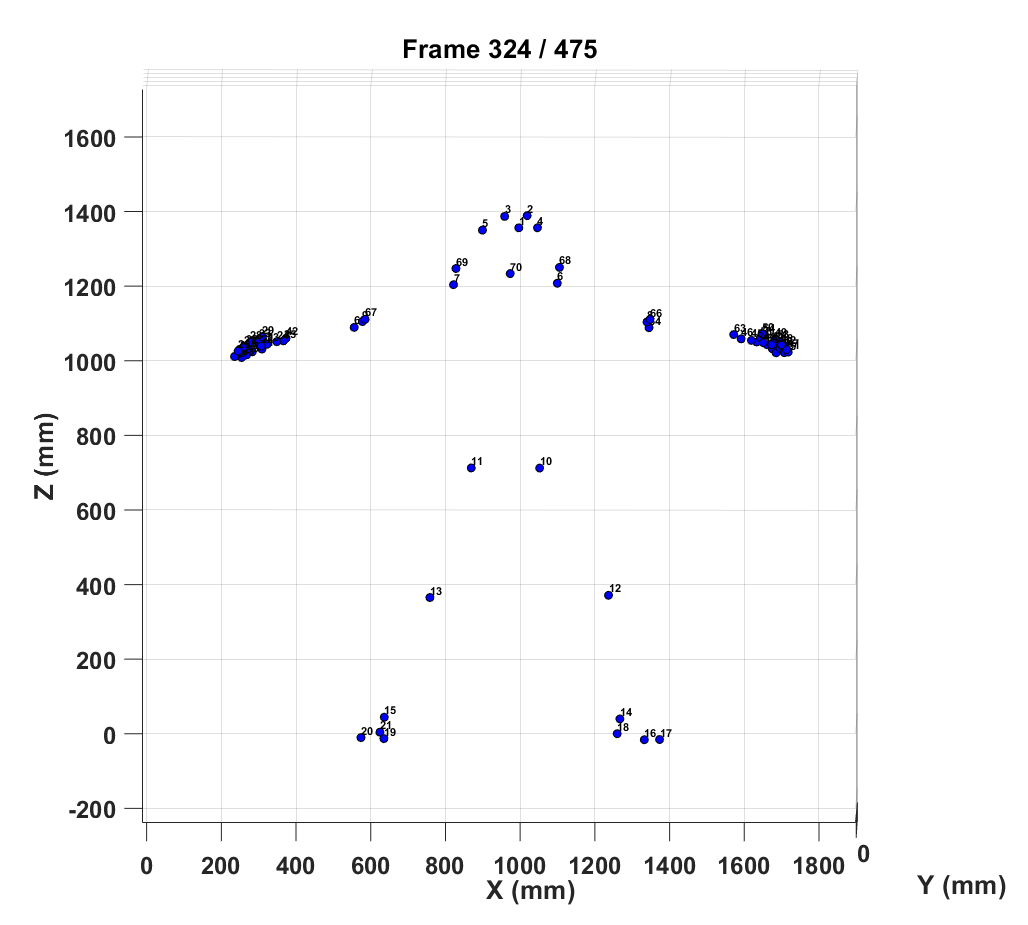
\includegraphics[width=\linewidth]{assets/Capture d'écran process/SAM 3D/modelSAM3D_2.png}
        \caption{Modèle 3D SAM 3D Body à la mauvaise échelle}
        \label{fig:sam3d_model}
    \end{subfigure}
    
    \caption{Problème d'échelle avec SAM 3D Body}
    \label{fig:SAM3D_scaleissues}
    \end{figure}
\end{itemize}

Des solutions auraient pu être développées pour corriger ces problèmes, mais avec le manque de temps, il a été décidé de s'arrêter à l'analyse angulaire des données 3D obtenues qui restent possibles malgré les problèmes cités précédemment. De la même façon que dans la partie \ref{estimation2D}, les angles articulaires ont été calculés et comparés aux données Vicon. L'objectif est maintenant de comparer les deux solutions - MoCapIA et SAM3D - à la méthode de référence Vicon afin d'identifier sur la méthode la plus performante. Les résultats montrent une erreur RMSE de $4.22^\circ$ pour le coude gauche et de $2.81^\circ$ pour le genou gauche soit des résultats équivalents à ceux de MoCapIA ($5.28^\circ$ et $2.74^\circ$ respectivement).

\begin{figure}[H]
    \centering
    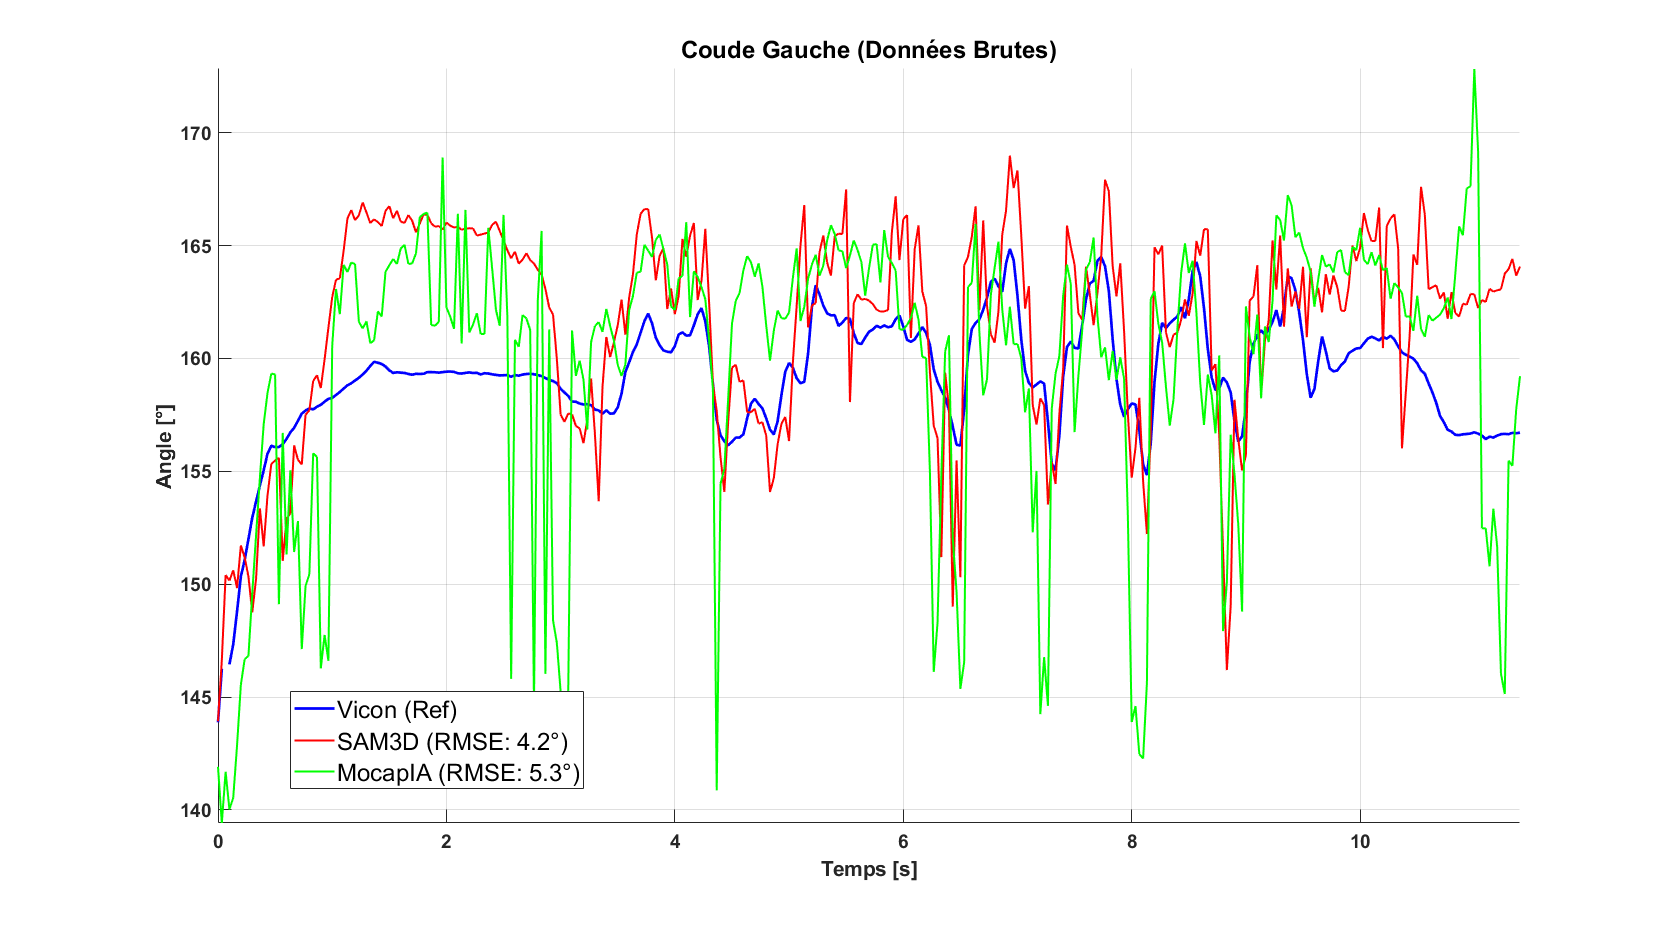
\includegraphics[width=\textwidth]{assets/Capture d'écran process/Vicon vs SAM3D vs MoCapIA/coudeG_vicon_sam3d_mocap.png}
    \caption{Comparaison à l'aide de la RMSE de l'angle du coude gauche entre Vicon, SAM 3D Body et MoCapIA}
    \label{fig:angle_coudeG_Vicon_SAM3D_MoCapIA}
\end{figure}

\begin{figure}[H]
    \centering
    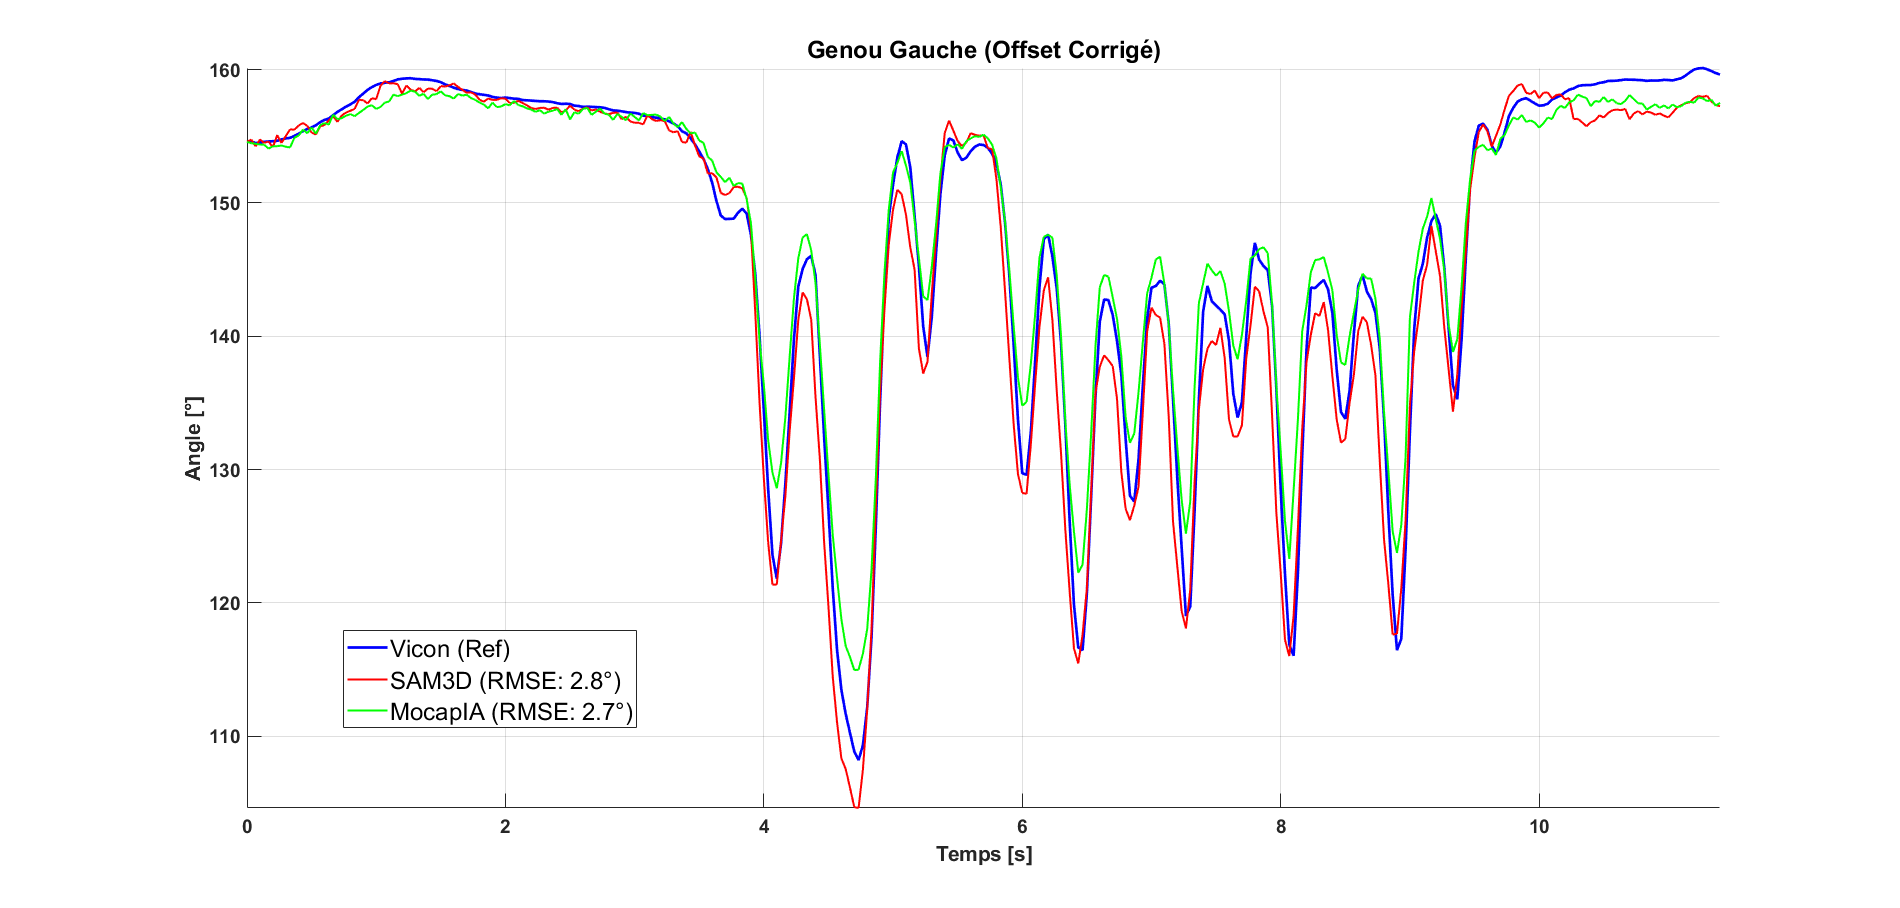
\includegraphics[width=\textwidth]{assets/Capture d'écran process/Vicon vs SAM3D vs MoCapIA/genouxG_vicon_sam3d_mocap.png}
    \caption{Comparaison à l'aide de la RMSE de l'angle du genou gauche entre Vicon, SAM 3D Body et MoCapIA}
    \label{fig:angle_genouG_Vicon_SAM3D_MoCapIA}
\end{figure}

Enfin une analyse de Bland-Altman a été réalisée pour valider ces résultats. Ils confirment ce qui vient d'être observé. En effet, pour le genou gauche (les autres articulations sont à retrouver en Annexe \ref{AnnexBlandAltmanSAM3D}), on observe que SAM 3D Body obtient des résultats similaires à MoCapIA avec un biais (une erreur systématique surement due au placement des marqueurs) de $-1.52^\circ$ et une variation aléatoire de $2.38^\circ$ contre un biais de $-0.97^\circ$ et une variation aléatoire de $2.54^\circ$ pour MoCapIA.

\begin{figure}[H]
    \centering
    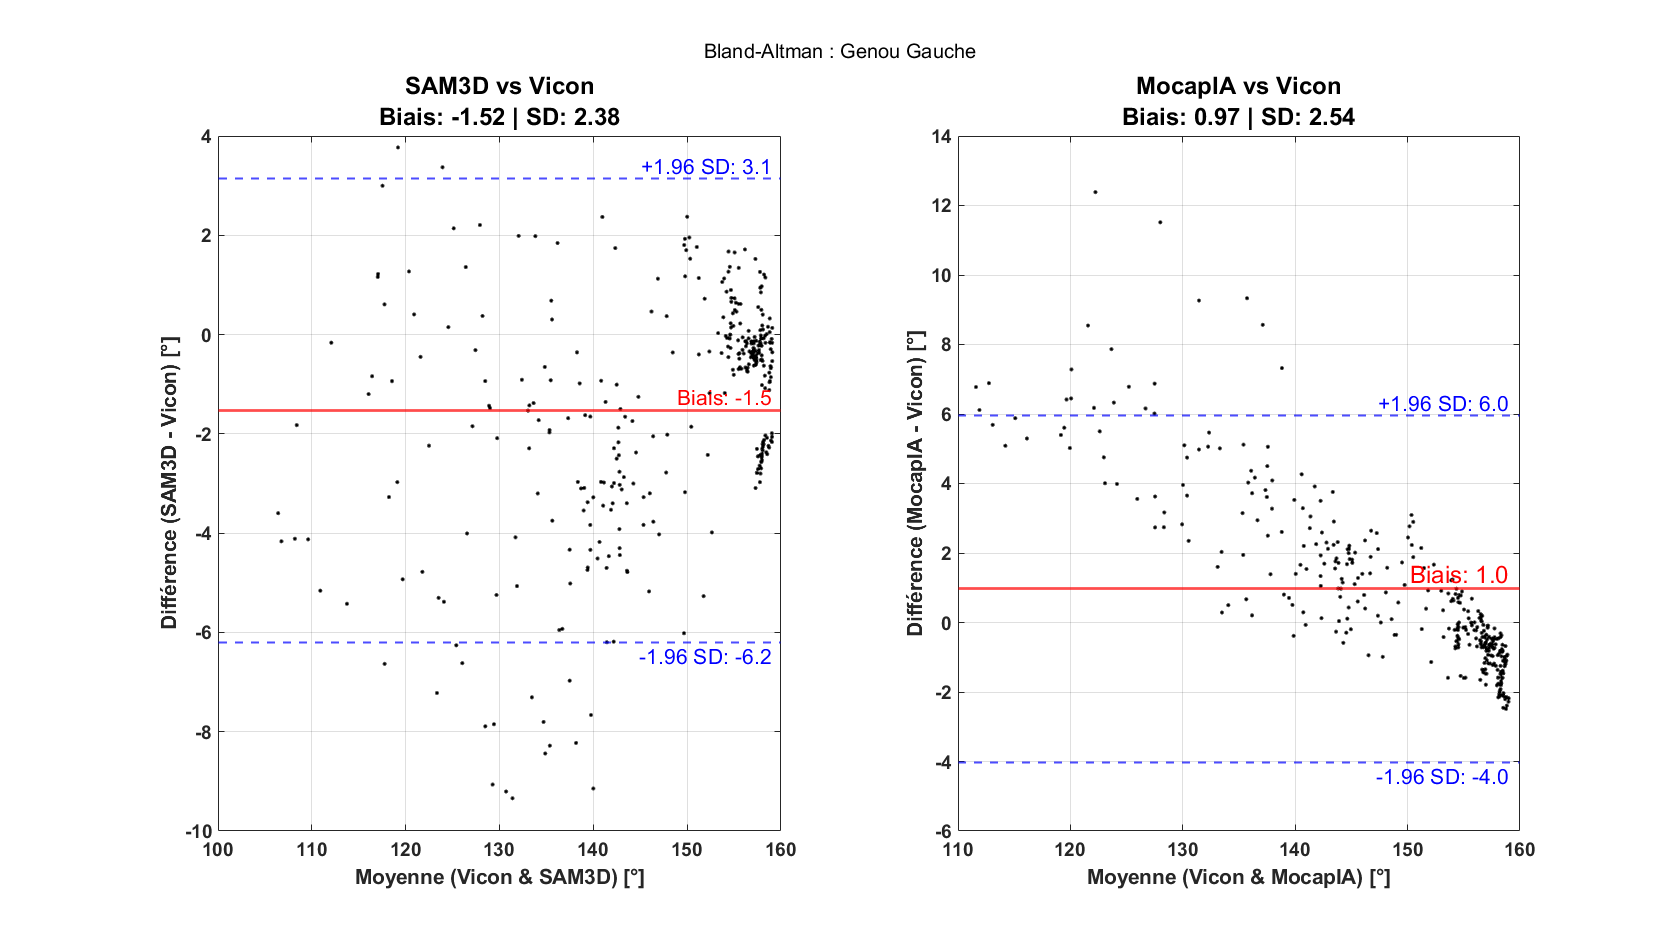
\includegraphics[width=\textwidth]{assets/Capture d'écran process/Vicon vs SAM3D vs MoCapIA/BlandAltman_Vicon_Mocap_sam3D.png}
    \caption{Analyse Bland-Altman entre Vicon, SAM 3D Body et MoCapIA pour le genou gauche}
    \label{fig:bland_altman_vicon_sam3d_mocapia}
\end{figure}

Même si les résultats sont légèrement meilleurs que MoCapIA, il est important de noter que les positions des points 3D de Sam 3D Body n'ont pas pu être comparées directement aux données Vicon et MoCapIA à cause des problèmes de référentiel et d'échelle. Ainsi, l'analyse angulaire seule ne permet pas de conclure définitivement sur la supériorité de SAM 3D Body par rapport à MoCapIA. Toutefois, ces résultats restent prometteurs pour une technologie aussi récente et pourraient faire partie des futures perspectives à donner au projet MoCapIA. 